\documentclass[11pt, a4paper]{article}

\usepackage[utf8]{inputenc}
\usepackage{fullpage}
\usepackage{graphicx}
\graphicspath{ {images/} }
\usepackage{color}
\usepackage{tabularx}
\usepackage{listings}
\usepackage{caption}
\usepackage{subcaption}
\usepackage{mathtools}
\usepackage{amssymb}
\usepackage{eurosym}
\usepackage[ngerman]{babel}
\usepackage[normalem]{ulem} %Squiggly underline
\usepackage{cancel} %Kürzen

\newcommand{\abs}[1]{\left\lvert#1\right\rvert}
\newcommand{\norm}[1]{\left\lVert#1\right\rVert}
\newcommand{\acos}{\mathrm{acos}}
\newcommand{\asin}{\mathrm{asin}}
\newcommand{\dx}{\ \mathrm{dx}}
\newcommand{\dt}{\ \mathrm{dt}}

\everymath{\displaystyle} %Force displaystyle everywhere

\lstset{
	tabsize=4,
	breaklines=true,
	showspaces=false
}

\title{Tutorium WS 14/15 \\ Lösungen}
\author{Christian Mielers}
\date{\today}

\begin{document}
\maketitle
\tableofcontents	

\newpage
\section{Höhere Mathematik}
\subsection{Wahrheitstabellen}
$(a \lor b) \lor (a \land b) \Leftrightarrow (a \lor b)$ \\
\begin{tabular}{|c|c|c|c|c|}
	\hline
	a & b & $\underline{a \lor b}$ & $a \land b$ & $\underline{(a \lor b) \lor (a \land b)}$ \vphantom{\Big(}\\
	\hline
  0 & 0 & 0 & 0 & 0\\
  0 & 1 & 1 & 0 & 1\\
  1 & 0 & 1 & 0 & 1\\
  1 & 1 & 1 & 1 & 1\\
   \hline
\end{tabular}

$(a \lor b) \land (a \lor \lnot b) \Leftrightarrow a \lor (b \land \lnot a)$ \\
\begin{tabular}{|c|c|c|c|c||c|c|c|c|}
	\hline
	a & b & $a \lor b$ & $a \lor \lnot b$ & $\underline{(a \lor b) \land (a \lor \lnot b)}$ &
	$\underline{a \lor (b \land \lnot a)}$ & $b \land \lnot a$ & a & b \vphantom{\Big(} \\
	\hline
	0 & 0 & 0 & 1 & 0 & 0 & 0 & 0 & 0\\
  0 & 1 & 1 & 0 & 0 & 1 & 1 & 0 & 1\\
  1 & 0 & 1 & 1 & 1 & 1 & 0 & 1 & 0\\
  1 & 1 & 1 & 1 & 1 & 1 & 0 & 1 & 1\\
  \hline
\end{tabular}

$\left((a \lor b) \Rightarrow (a \land b) \right) \Leftrightarrow (a \land b) \lor (\lnot a \land \lnot b)$ \\
\begin{tabular}{|c|c|c|c|c||c|c|}
	\hline
	a & b & $a \lor b$ & $a \land b$ & $\underline{(a \lor b) \Rightarrow (a \land b)}$ &
	$\underline{(a \land b) \lor (\lnot a \land \lnot b)}$ & $\lnot a \land \lnot b$ \vphantom{\Big(} \\
	\hline
  0 & 0 & 0 & 0 & 1 & 1 & 1\\
  0 & 1 & 1 & 0 & 0 & 0 & 0\\
  1 & 0 & 1 & 0 & 0 & 0 & 0\\
  1 & 1 & 1 & 1 & 1 & 1 & 0\\
  \hline
\end{tabular}

\subsection{Mengenlehre}
Gelten die folgenden Beziehungen für beliebige Mengen X, Y und Z?
\begin{enumerate}
	\item $X \setminus (Y \cap Z) = (X \setminus Y) \cap (X \setminus Z)$
	\begin{figure}[h!]
		\centering
		\begin{subfigure}{3cm}
			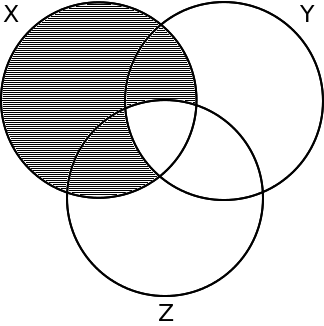
\includegraphics[height=3cm]{MengenlehreAufgabe1a}
			\caption{Linke Seite}
		\end{subfigure}
		\begin{subfigure}{3cm}
			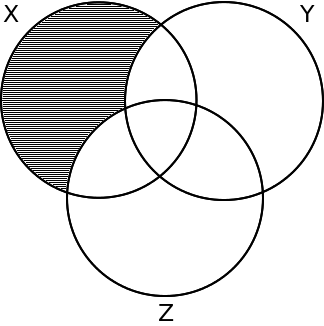
\includegraphics[height=3cm]{MengenlehreAufgabe1b}
			\caption{Rechte Seite}
		\end{subfigure}
	\end{figure} \\
	Gegenbeispiel finden: $X \cup Y$ oder $X \cup Z$ darf nicht leer sein. \\
	Sei $X = \{1,2,3\}, Y = \{2,4,6\}$ und $Z = \{7,8,9\}$ \\
	Dann ist $X \setminus (Y \cap Z) = \{1,2,3\} \quad \neq \quad \{1,3\} = (X \setminus Y) \cap (X \setminus Z)$
	\item $(X \cup Y) \setminus Z = \big((X \setminus Z) \cup (Y \setminus Z)\big) \setminus (Y \cap Z)$
	\begin{figure}[h!]
		\centering
		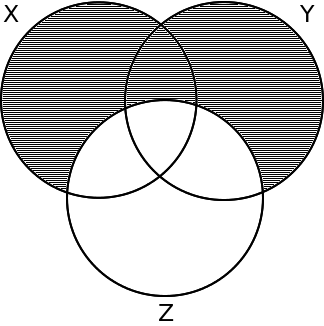
\includegraphics[height=3cm]{MengenlehreAufgabe2}
		\caption{linke / rechte Seite}
	\end{figure} \\
	\begin{align*}
		(X \cup Y) \setminus Z &= \big((X \setminus Z) \cup (Y \setminus Z)\big) \setminus (Y \cap Z) \\
		(X \cup Y) \setminus Z &= (X \setminus Z) \cup (Y \setminus Z) \\
		(X \setminus Z) \cup (Y \setminus Z) &= (X \setminus Z) \cup (Y \setminus Z)
	\end{align*}
\end{enumerate}

\subsection{Abbildungen}
Sind die folgenden Funktionen injektiv, surjektiv, bijektiv?
\begin{enumerate}
	\item $\mathrm{f}(x) = x^4+2 \qquad \mathrm{f}: \mathrm{R} \mapsto \mathrm{R}$ \\
	nicht injektiv: $\mathrm{f}(1) = \mathrm{f}(-1)$ \\
	nicht surjectiv: $\forall x: \mathrm{f}(x) \geq 2$. Alternativ: $\nexists x: \mathrm{f}(x) = 0$ \\
	Somit ist f nicht bijektiv.
	\item $\mathrm{f}(x) = x^4+2 \qquad \mathrm{f}: \mathrm{R} \mapsto (2, + \infty)$ \\
	nicht injektiv: $\mathrm{f}(1) = \mathrm{f}(-1)$ \\
	surjektiv: $\mathrm{f}(x) = x^4 + 2 \Leftrightarrow \sqrt[4]{\mathrm{f}(x) - 2} = x$ \\
	$\sqrt[4]{\mathrm{f(x)}-2}$ existiert eindeutig für $x \geq 2$ (und somit auch für $x > 0$) \\
	Somit ist f nicht bijektiv.
	\item $\mathrm{f}(x) = x^3+1 \qquad \mathrm{f}: \mathrm{R} \mapsto \mathrm{R}$ \\
	injektiv: $x^3 + 1 = y^3 + 1 \Rightarrow x^3 = y^3 \Rightarrow x = y$ (Technischer: $\nexists x \neq y: x^3 + 1 \neq x^3 + 1$) \\
	surjektiv: $\forall y \in \mathrm{R}: \exists x \in \mathrm{R}: y = x^3 + 1 \Leftrightarrow y - 1 = x^3 \Leftrightarrow \sqrt[3]{y-1} = x$
	Somist ist f bijektiv.
	\item $\mathrm{f}(x) = \sin(x) \qquad \mathrm{f}: \mathrm{R} \mapsto [-1, 1]$ \\
	nicht injektiv: $\sin(\pi) = \sin(2 \pi)$ \\
	surjektiv: $\sin\left(-\frac{\pi}{2}\right) = -1$, $\sin\left(\frac{\pi}{2}\right) = 1$ und $\sin(x)$ steigt auf dem stetigen Intervall $\left[-\frac{\pi}{2},-\frac{\pi}{2}\right]$ monoton. \\
	Somit ist f nicht bijektiv.
	\item $\mathrm{f}(x) = x^4 - x^2 \qquad \mathrm{f}: \mathrm{R} \mapsto \mathrm{R}$ \\
	nicht injektiv: $\mathrm{f}(1) = \mathrm{f}(-1)$ \\
	nicht surjektiv: $\nexists x: \mathrm{f}(x) = 0$ \\
	Somit ist f nicht bijektiv.
	\item $\mathrm{f}(x) = \frac{1}{x} \qquad \mathrm{f}: \mathrm{R} \mapsto \mathrm{R}$ \\
	injektiv: Sei $x \neq y$. Dann $\frac{1}{x} \neq \frac{1}{x}$ \\
	nicht surjektiv: $\nexists x \in \mathrm{R}: \frac{1}{x} = 0$ \\
	Somit ist f nicht bijektiv.
\end{enumerate}
Invertiere folgende Funktionen:

Zum invertieren tausche x und f(x) bzw. x und y und löse nach f(x) bzw. y auf. Bei Schrittweise definierten Funktionen müssen auch die Grenzen angepasst werden!
\begin{enumerate}
	\item $\mathrm{f}(x) = x^3 \qquad \mathrm{f}: \mathrm{R} \mapsto \mathrm{R}$ \\
	$x = {\mathrm{f}(x)}^3$ \\
	$\sqrt[3]{x} = f(x)$
	\item $\mathrm{f}(x) = \frac{1}{x} \qquad \mathrm{f}: \mathrm{R} \setminus \{0\} \mapsto \mathrm{R} \setminus \{0\}$ \\
	$x = \frac{1}{\mathrm{f}(x)}$ (Vertauschen von f(x) und x)\\
	$\mathrm{f}(x) = \frac{1}{x}$ (Aufgelöst nach f(x))
	\item $\mathrm{f}(x) =
		\begin{cases}
			-\frac{1}{2}x + 3 & x \in (-\infty, 4) \\
			-3x + 13 & x \in [4, +\infty)
		\end{cases}
		$
		\begin{enumerate}
			\item $\mathrm{f}(x) = -\frac{1}{2}x + 3$ invertieren \\
				\begin{align*}
					x &= -\frac{1}{2}\mathrm{f}(x) + 3 \\
					x-3 &= -\frac{1}{2}\mathrm{f}(x) \\
					-2x+6 &= \mathrm{f}(x)
				\end{align*}
			\item $\mathrm{f}(x) = -3x + 13$ invertieren
			\begin{align*}
				x = -3 \mathrm{f}(x) + 13 \\
				x - 13 = -3 \mathrm{f}(x) \\
				\frac{-x + 13}{3} = \mathrm{f}(x)
			\end{align*}
			\item Grenzen neu berechnen \\
			y-Wert des Schnittpunktes in Umkehrfunktion der Funktion einsetzen, die den Schnittpunkt enthält: \\
			$\mathrm{f}(1) = \frac{-1 + 13}{3} = 4$ \\
			Der neue Schnittpunkt hat also die Koordinaten (1,4)
		\end{enumerate}
		Die Umkehrfunktion ist somit:
		$\begin{cases}
			-2x+6, & x \in (-\infty,1) \\
			\frac{-x + 13}{3} & x \in [1, +\infty)
		\end{cases}$
\end{enumerate}

\subsection{Algebraische Strukturen}
Sind folgende Mengen-Abbildungspaare Gruppen, Ringe, Körper oder nichts davon?

Eine Algebraische Struktur kann (u.A.) folgende Eigenschaften aufweisen:
\begin{description}
	\item[A1] Assoziativität (Addition)
	\item[A2] Kommutativität (Addition)
	\item[A3] Neutrales Element (Addition)
	\item[A4] Inverses Element (Addition)
	\item[M1] Assoziativität (Multiplikation)
	\item[M2] Kommutativität (Multiplikation)
	\item[M3] Neutrales Element (Multiplikation)
	\item[M4] Inverses Element (Multiplikation)
	\item[D] Distributivität
\end{description}
Sind A1 - A4 erfüllt handelt es sich um eine Kommutative Gruppe, bei A1-M2 und D um einen Kommutativen Ring und ein Körper ist die Struktur dann, wenn alle Eigenschaften erfüllt sind.

\begin{enumerate}
	\item $\left( \mathbb{N}_0, + \right)$ ist nichts \\
	Kein inverses Element bzgl. +: $\nexists x \in \mathbb{N}_0: 3+x=0$
	\item $\left( \mathbb{Z}, + \right)$ ist eine Gruppe \label{ZGruppe} \\
	Addition ist Assoziativ \\
	Addition ist Kommutativ \\
	0 ist das neutrale Element der Addition und $0 \in \mathbb{Z}$ \\
	Das inverse Element zu a ist $-a$
	\item $\left( \mathbb{Z}, +, \cdot \right)$ ist ein Ring \label{ZRing} \\
	Axiome für die Addition gelten (siehe \ref{ZGruppe}.) \\
	Multiplikation ist Assoziativ: $(a \cdot b) \cdot c = a \cdot (b \cdot c)$ \\
	Multiplikation ist Kommutativ: $a \cdot b = b \cdot a$ \\
	Das Distributivgesetzt gilt für Addition und Multiplikation: $a(b+c) = ab + ac$ \\ \\
	Aber: $\left( \mathbb{Z}, +, \cdot \right)$ ist kein Körper! \\
	Es gibt zwar ein neutrales Element der Multiplikation (die 1), aber es gibt nicht für jedes Element eine Inverse, für die 3 z.B. nicht: $\nexists x \in \mathbb{Z}: 3\cdot x = 1$
	\item $\left( \mathbb{R}, +, \cdot \right)$ ist ein Körper \\
	Axiome für Addition gelten (siehe \ref{ZGruppe}.) \\
	Assoziativität und Kommutativität der Multiplikation gelten (siehe \ref{ZRing}.) \\
	Distributivität gilt (siehe \ref{ZRing}.) \\
	1 ist das neutrale Element der Multiplikation. \\
	Das inverse Element zu a ist $\frac{1}{a}$ (und jeder Bruch ist $\in \mathbb{R}$).
	\item $\left( \mathrm{M}, +, \cdot \right)$ mit $\mathrm{M} = \{ -2,0,\frac{1
	}{2},1,2 \}$ ist nichts \\
	Verletzung der Abgeschlossenheit: $1+2 \notin \mathrm{M}$, somit gilt nicht: $\mathrm{M} \times \mathrm{M} \mapsto \mathrm{M}$ \\
	Kein additives Inverses zu 1: $\nexists x \in \mathrm{M}: 1+x=0$ \\
	Kein multiplikatives Inverses zu -2: $\nexists x \in \mathrm{M}: -2 \cdot x = 1$
	\item $\left( \mathbb{R}, +, \circ \right)$ mit $a \circ b = 3a + b$ ist nichts \\
	$\circ$ ist nicht assoziativ:
	\begin{align*}
		(a \circ b) \circ c &= a \circ (b \circ c) \\
		(3a + b) \circ c &= a \circ (3b + c) \\
		3(3a + b) + c &= 3a + (3b + c) \\
		9a + 3b + c &= 3a + 3b + c \\
		9a &\neq 3a
	\end{align*}
\end{enumerate}

\subsubsection{Kommutative Gruppen}
Zeige, dass $(G,*)$ eine kommutative Gruppe ist mit $G=\mathbb{R} \setminus \{1\}$ und $x * y = x+y-xy$. Was ist das neutrale Element, und wie bildet sich das inverse Element?
\begin{enumerate}
	\item[(A1)] $(x * y) * z = x * (y * z)$
		\begin{align*}
			(x+y-xy) * z &= x * (y+z-yz) \\
			x+y-xy + z - z(x+y-xy) &= x+ y+z-yz - x(y+z-yz) \tag*{$-x-y-z$} \\
			-xy - (zx+zy-xyz)&= -yz - (xy+xz-xyz) \\
			-xy - zx - zy + xyz &= -yz - xy - xz + xyz \tag*{- xyz + xy} \\
			- zx - zy &= -yz - xz \tag*{sichtbar gleich}
		\end{align*}
	\item[(A2)] $x * y = y * x$
		\begin{align*}
			x+y-xy &= y+x-xy \\
			x+y-xy &= x+y-xy
		\end{align*}
	\item[(A3)] $"0" * x = x$ (neutrales Element, hier n)
		\begin{align*}
			n * x &= x \\
			n+x-nx &= x \\
			\underbrace{(1-n)}_{=1}x &= x \\
			n &= 0
		\end{align*}
	\item[(A4)] $x * (-x) = 0$ bzw. $x * i = n$
		\begin{align*}
			x + i - xi &= 0 \\
			i - xi &= -x \\
			(1-x)i &= -x \\
			i &= \frac{-x}{1-x} \tag*{$1 \notin G$} \\
			i &= \frac{x}{x-1}
		\end{align*}
\end{enumerate}

\subsubsection{Körper}
Vervollständige folgende Tabellen für den Körper $K = \left\{\{0,1,a,b,c\right\}, +, \cdot\} $. 0 ist das neutrale Element der Addition, 1 der Multiplikation
\begin{center}
	\begin{tabular}{c|ccccc}
		+ & 0 & 1 & a & b & c \\ \hline
		0 & 0 & 1 & a & b & c \\
		1 & 1 & a & b & c & 0 \\
		a & a & b & c & 0 & 1 \\
		b & b & c & 0 & 1 & a \\
		c & c & 0 & 1 & a & b \\
	\end{tabular}
	\hspace{2cm}
	\begin{tabular}{c|ccccc}
		$\cdot$ & 0 & 1 & a & b & c \\ \hline
		0 & 0 & 0 & 0 & 0 & 0 \\
		1 & 0 & 1 & a & b & c \\
		a & 0 & a & c & 1 & b \\
		b & 0 & b & 1 & c & a \\
		c & 0 & c & b & a & 1 \\
	\end{tabular}
\end{center}
$a \equiv 2, \quad b \equiv 3, \quad c \equiv 4$ \\
Was ist das inverse Element von b in K bzgl. der Multiplikation? \\
Finde x so dass $a \cdot b \cdot x = a$ bzw. $b \cdot x = 1$. Die Inverse von $b$ ist also a: $b^{-1} = a$

\begin{center}
	\begin{tabular}{c|ccccc}
		+ & 0 & 1 & a & b & c \\ \hline
		0 & 0 & 1 & a & b & c \\
		1 & 1 & b & 0 & c & a \\
		a & a & 0 & c & 1 & b \\
		b & b & c & 1 & a & 0 \\
		c & c & a & b & 0 & 1 \\
	\end{tabular}
	\hspace{2cm}
	\begin{tabular}{c|ccccc}
		$\cdot$ & 0 & 1 & a & b & c \\ \hline
		0 & 0 & 0 & 0 & 0 & 0 \\
		1 & 0 & 1 & a & b & c \\
		a & 0 & a & 1 & c & b \\
		b & 0 & b & c & a & 1\\
		c & 0 & c & b & 1 & a \\
	\end{tabular}
\end{center}
$a \equiv 4, \quad b \equiv 2, \quad c \equiv 3$

\subsection{Summen und Produkte}
Berechne folgende Summen:
\begin{enumerate}
	\item $\sum_{i=2}^{15} 4 = 56$
	\item $\sum_{i=0}^5 i^3 = 0 + 1 + 8 + 27 + 64 + 125 = 225$
	\item $\sum_{i=0}^5 (-1)^i (4i+3) = 3-7+11-15+19-23 = -12$
\end{enumerate}
Berechne folgende Produkte:
\begin{enumerate}
	\item $\prod_{i=1}^7 i = 1 \cdot 2 \dots 6 \cdot 7 = 5040$
	\item $\prod_{i=1}^4 \frac{i}{2} = \frac{1}{2} \cdot \frac{2}{2} \cdot \frac{3}{2} \cdot \frac{4}{2} = \frac{24}{2^4} = \frac{3}{2}$
	\item $\prod_{i=1}^4 \frac{3i^2+2}{i} = \frac{5}{1} \cdot \frac{14}{2} \cdot \frac{29}{3} \cdot \frac{50}{4} = 5 \cdot 7 \cdot \frac{29}{3} \cdot \frac{25}{2} = \frac{25375}{6}$
\end{enumerate}

\subsection{Binomialkoeffizient}
$\binom{n}{k} = \frac{n!}{k!(n-k)!}$ \\
Welchen Wert hat n?
\begin{enumerate}
	\item $ n = \binom{6}{3} = \frac{6!}{3!(6-3)!} = \frac{\cancel{1\cdot2\cdot3}\cdot4\cdot5\cdot6}{\cancel{(1\cdot2\cdot3)}3!} = \frac{4\cdot5\cdot\cancel{6}}{1\cdot\cancel{2\cdot3}} = 4\cdot5 = 20$
	\item $n = \binom{10}{7} = \frac{10!}{7!(10-7)!} = \frac{8 \cdot 9 \cdot 10}{3!} = \frac{720}{6} = 120$
	\item $\binom{n+3}{n+1} + \binom{n+4}{n+2} + \binom{n-1}{n-3} = 70$
		\begin{align*}
			\binom{n+3}{2} + \binom{n+4}{2} + \binom{n-1}{2} &= 70 \\
			\frac{(n+3)!}{2!(n+3-2)!} + \frac{(n+4)!}{2!(n+4-2)!} + \frac{(n-1)!}{2!(n-1-2)!} &= 70 \tag{Definition} \\
			\frac{(n+3)!}{2(n+1)!} + \frac{(n+4)!}{2(n+2)!} + \frac{(n-1)!}{2(n-3)!} &= 70 \\
			\frac{(n+3)!}{(n+1)!} + \frac{(n+4)!}{(n+2)!} + \frac{(n-1)!}{(n-3)!} &= 140 \tag{Kürzen} \\
			(n+2)(n+3) + (n+3)(n+4) + (n-2)(n-1) &= 140 \\
			n^2+5n+6 + n^2+7n+12 + n^2-3n+2 &= 140 \\
			3n^2+9n-120 &= 0 \\
			n^2+3n-40 &= 0 \tag{PQ-Formel} \\
			x_1 = -8, \quad x_2 &= 5 \tag{Probe!}
		\end{align*}
		Der Einfache Binomialkoeffizient ist nur für positive Zahlen definiert, die Lösung ist also $x=1$.
\end{enumerate}

\subsection{Ordnungsrelationen}
Ergänze bei folgenden Ausdrücken die Relationszeichen $\subset, \subseteq, \supseteq, \supset,$ \\
\begin{tabular}{|l|c|l|}
	\hline
	Menge 1 & \hspace{3mm} ? \hspace{3mm} & Menge 2 \\ \hline
	$\{1,2,3\}$ & $\subseteq, \supseteq$ & $\{1,2,3\}$ \\
	$\{5,6\}$ & $\subset$ & $\{5,6,7,8\}$ \\
	$\{\sqrt{2}, \pi, 3\}$ & nichts & $\mathbb{R}$ \\
	$\mathbb{R}$ & $\supset$ & $\mathbb{Q} \setminus {\pi, e}$ \\
	$\mathbb{N}_0$ & $\supset$ & $\mathbb{N}$ \\
	$\mathbb{I}$ & $\subset$ & $\mathbb{R}$ \\
	$\mathbb{C} \setminus \mathbb{I}$ & nichts & $\left(\mathbb{Q} \setminus \mathbb{N}\right) \cup \{2,4,6\}$ \\ \hline
\end{tabular}

\subsection{Ungleichungen}
Für welche $x$ gelten die folgenden Ungleichungen?
\begin{enumerate}
	\item $5x-3 < \dfrac{2x^2+3x}{x}$
		\begin{align*}
			5x-3 &< 2x+3 \\
			3x &< 6 \\
			x &< 2
		\end{align*}
	\item $\dfrac{x+1}{2} \geq \abs{2x-3}$
		\begin{align*}
			\dfrac{x+1}{2} &\geq 2 \abs{x-\frac{3}{2}}
			\shortintertext{Fall 1: $x \in \left(-\infty, \frac{3}{2}\right)$}
			\dfrac{x+1}{2} &\geq 2 (-1) \left(x-\frac{3}{2}\right) \\
			\dfrac{x+1}{2} &\geq 2 \left(\frac{3}{2} - x\right) \\
			\dfrac{x+1}{2} &\geq 3 - 2x \\
			x+1 &\geq 6 - 4x \\
			5x &\geq 5 \\
			x &\geq 1
			\intertext{Also Lösung im Fall 1: $x \in \left(-\infty, \frac{3}{2}\right) \cap \left[1,+\infty\right) = \left[ 1, \frac{3}{2} \right)$}
			\shortintertext{Fall 2: $x \in \left[ \frac{3}{2}, +\infty \right)$}
			\dfrac{x+1}{2} &\geq 2 \left(x-\frac{3}{2}\right) \\
			x+1 &\geq 4x - 6 \\
			7 &\geq 3x \\
			\frac{7}{3} &\geq x
			\intertext{Also Lösung im Fall 2: $x \in \left[ \frac{3}{2}, +\infty \right) \cap \left( -\infty, \frac{7}{3} \right] = \left[ \frac{3}{2}, \frac{7}{3} \right]$}
		\end{align*}
		Das Gesammtergebnis ergibt sich also aus $\left[ 1, \frac{3}{2} \right) \cup \left[ \frac{3}{2}, \frac{7}{3} \right] = \left[ 1, \frac{7}{3} \right]$
	\item $\sqrt{x^2-2x+1} > 3 - \abs{x-2}$
		\begin{align*}
			\sqrt{(x-1)^2} &> 3 - \abs{x-2} \\
			\abs{x-1} &> 3 - \abs{x-2}
			\shortintertext{Fall 1: $x \in \left( -\infty, 1 \right )$}
			(-1)(x-1) &> 3 + x-2 \\
			1-x &> 3 + x-2 \\
			0 &> 2x \\
			0 &> x
			\intertext{Also Lösung im Fall 1: $x \in \left( -\infty, 1 \right ) \cap \left( -\infty, 0 \right) = \left( -\infty, 0 \right)$}
			\shortintertext{Fall 2: $x \in \left[ 1, 2 \right)$}
			x-1 &> 3 + (x-2) \\
			x > &2 + x \\
			0 &> 2
			\intertext{Also Lösung im Fall 2: $x \in \left[ 1, 2 \right) \cap \emptyset = \emptyset$ (Fall 2 hat keine Lösung!)}
			\shortintertext{Fall 3: $x \in \left[ 2, +\infty \right)$}
			x-1 &> 3 - (x-2) \\
			x-1 &> 3 - x + 2 \\
			2x &> 6 \\
			x &> 3
			\intertext{Also Lösung im Fall 3: $x \in \left[ 2, +\infty \right) \cap \left( 3, +\infty \right) = \left( 3, +\infty \right)$}
		\end{align*}
		Das Gesammtergebnis ergibt sich also aus $\left( -\infty, 0 \right) \cup \left( 3, +\infty \right).$
	\item $\sqrt{x^2-8x+16} < \frac{\abs{x+2}}{2}$
		\begin{align*}
			\sqrt{x^2-8x+16} &< \frac{\abs{x+2}}{2} \\
			2 \abs{x-4} &< \abs{x+2}
			\shortintertext{Fall 1: $x \in (-\infty, -2)$}
			2 (-x+4) &< -x-2 \\
			-2x+8 &< -x-2 \\
			10 &< x
			\intertext{Also Lösung im Fall 1: $x \in (10, +\infty) \cap (-\infty, -2) = \emptyset$ (Fall 1 hat keine Lösung!)}
			\shortintertext{Fall 2: $x \in [-2, 4)$}
			2 (-x+4) &< x+2 \\
			-2x+8 &< x+2 \\
			6 &< 3x \\
			2 &< x
			\intertext{Also Lösung im Fall 2: $x \in (2, +\infty) \cap [-2, 4) = (2,4)$}
			\shortintertext{Fall 3: $x \in [4, +\infty]$}
			2 (x-4) &< x+2 \\
			2x-8 &< x+2 \\
			x &< 10
			\intertext{Also Lösung im Fall 3: $x \in (-\infty, 10) \cap [4, +\infty) = [4,10)$}
		\end{align*}
		Das Gesammtergebnis ergibt sich also aus $(2,4) \cup [4,10) = (2,10).$
	\item $\sqrt{x^2-2x+1} > 3 + \abs{x-2}$
		\begin{align*}
			\abs{x-1} &> 3 + \abs{x-2} \\
			\abs{x-1} - \abs{x-2} &> 3
		\end{align*}
		Die Ungleichung hat keine Lösung.
\end{enumerate}

\subsection{Induktion}
Beweise per vollständiger Induktion:
\begin{enumerate}
	\item $\forall n \geq 1 : \sum_{i=1}^n i = \frac{n(n+1)}{2}$ (Gauß'sche Summenformel)
		\begin{description}
			\item[Anfang] $n=1$
				\begin{align*}
					\sum_{i=1}^1 1 &= \frac{1(1+1)}{2} \\
					1 &= \frac{2}{2}
				\end{align*}
			\item[Annahme] $\sum_{i=1}^n i = \frac{n(n+1)}{2}$
			\item[Schritt] 
			\begin{align*}
				\sum_{i=1}^{n+1} i &= \frac{(n+1)(n+2)}{2} \\
				n+1 + \sum_{i=1}^n i &= \frac{(n+1)(n+2)}{2} \\
				n+1 + \frac{n(n+1)}{2} &= \frac{(n+1)(n+2)}{2} \\
				n+1 + \frac{n^2 + n}{2} &= \frac{n^2 + 3n + 2}{2} \\
				\frac{2n+2}{2} + \frac{n^2 + n}{2} &= \frac{n^2 + 3n + 2}{2} \\
				\frac{n^2 + 3n + 2}{2} &= \frac{n^2 + 3n + 2}{2}
			\end{align*}
		\end{description}
	\item $\forall n \geq 1 : \sum_{i=1}^n (2i-1) = n^2$ (Summe ungerader Zahlen)
		\begin{description}
			\item[Anfang] $n=1$
				\begin{align*}
					\sum_{i=1}^1 (2i-1) &= 1^2 \\
					2 \cdot 1-1 &= 1 \\
					1 &= 1
				\end{align*}
			\item[Annahme] $\sum_{i=1}^n (2i-1) = n^2$
			\item[Schritt] 
				\begin{align*}
					\sum_{i=1}^{n+1} (2i-1) &= (n+1)^2 \\
					2(n+1) - 1 + \sum_{i=1}^n (2i-1) &= (n+1)^2 \\
					2(n+1) - 1 + n^2 &= (n+1)^2 \\
					n^2+2n+1 &= (n+1)^2 \\
					(n+1)^2 &= (n+1)^2
				\end{align*}
		\end{description}
	\item $\forall n \geq 1 : \sum_{i=1}^n (2i-1)^2 = \frac{n (2n-1)(2n+1)}{3}$
		\begin{description}
			\item[Anfang] $n=1$
				\begin{align*}
					\sum_{i=1}^1 (2i-1)^2 = \frac{1 (2 \cdot 1-1)(2 \cdot 1 +1)}{3} \\
					(2 \cdot 1-1)^2 = \frac{1 \cdot 3}{3} \\
					1 = 1
				\end{align*}
			\item[Annahme] $\sum_{i=1}^n (2i-1)^2 = \frac{n (2n-1)(2n+1)}{3}$
			\item[Schritt] 
				\begin{align*}
					\sum_{i=1}^{n+1} (2i-1)^2 &= \frac{(n+1) (2(n+1)-1)(2(n+1)+1)}{3} \\
					(2(n+1)-1)^2 + \sum_{i=1}^n (2i-1)^2 &= \frac{(n+1)(2n+1)(2n+3)}{3} \\
					(2n+1)^2 + \frac{n(2n-1)(2n+1)}{3} &= \frac{(n+1)(2n+1)(2n+3)}{3} \\
					3(4n^2+4n+1) + n(2n-1)(2n+1) &= (n+1)(2n+1)(2n+3) \\
					12n^2+12n+3 + (2n^2-n)(2n+1) &= (2n^2+3n+1)(2n+3) \\
					12n^2+12n+3 + (4n^3-n) &= 4n^3+12n^2+11n+3 \\
					4n^3+12n^2+11n+3 &= 4n^3+12n^2+11n+3
				\end{align*}
		\end{description}
	\item $\forall n \geq 1 : \quad 3 \mid (n^3 - n)$
		\begin{description}
			\item[Anfang] $n=1$
				\begin{align*}
					3 &\mid (1^3 - 1) \\
					3 &\mid 0
				\end{align*}
			\item[Annahme] $3 \mid (n^3 - n)$
			\item[Schritt] 
			\begin{align*}
				3 &\mid (n+1)^3 - (n+1) \\
				3 &\mid (n^2+2n+1)(n+1) - n-1) \\
				3 &\mid (n^3+3n^2+3n+1) - n-1) \\
				3 &\mid n^3+3n^2+2n \\
				3 &\mid (n^2+3n+2)n \\
				3 &\mid (n-2)(n-1)n \\
				3 &\mid (n-2) \lor 3 \mid (n-1) \lor 3 \mid n
			\end{align*}
		\end{description}
	\item $\forall n \geq 4 : \quad 2^n \geq n^2$
		\begin{description}
			\item[Anfang] $n=4$
				\begin{align*}
					2^4 &\geq 4^2 \\
					16 &\geq 16
				\end{align*}
			\item[Annahme] $2^n \geq n^2$
			\item[Schritt] 
				\begin{align*}
					2^{n+1} &\geq (n+1)^2 \\
					2 \cdot 2^n &\geq n^2 + 2n + 1 \tag{Verwende Annahme} \\
					2 n^2 &\geq n^2 + 2n + 1 \tag{$- n^2$} \\
					n^2 &\geq 2n + 1 \\
					n^2 -2n - 1 &\geq 0 \tag{Zerlegung in Linearfaktoren} \\
					(n-1-\sqrt{2})(n-1+\sqrt{2}) &\geq 0 \tag{Beide Terme $\geq 0$ weil $n \geq 4$}
				\end{align*}
		\end{description}
\end{enumerate}

\subsection{Einheitskreis}
\begin{figure}[h!]
	\centering
	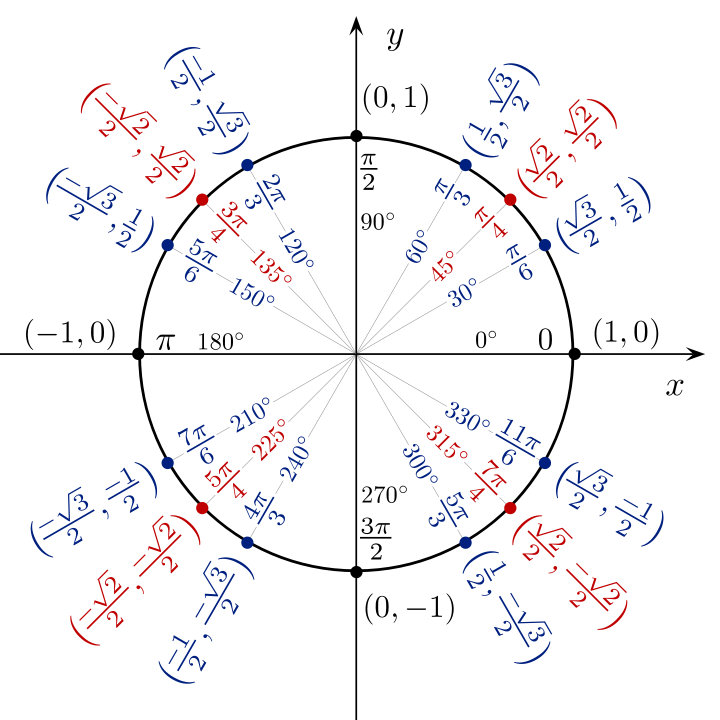
\includegraphics[height=\textwidth]{Einheitskreis.png}
	\caption{Einheitskreis: (cos, sin)}
	\label{einheitskreis}
\end{figure}
Lese aus dem Einheitskreis (Abbildung \ref{einheitskreis}) ab:
\begin{enumerate}
	\item $\cos \frac{\pi}{4} = \frac{\sqrt{2}}{2}$
	\item $\sin \frac{5\pi}{4} = -\frac{\sqrt{2}}{2}$
	\item $\acos -\frac{\sqrt{3}}{2} = \frac{5\pi}{6} \text{ bzw. } \frac{7\pi}{6}$
	\item $\asin -\frac{1}{2} = \frac{7\pi}{6} \text{ bzw. } \frac{11\pi}{6}$
\end{enumerate}

\subsection{Komplexe Zahlen}
Gegeben seien folgende Zahlen $\in \mathbb{C}$. Bestimme den Real- und Imaginärteil, die komplex konjugierte so wie den Betrag: \\
Betrag: $\abs{x+yi} = \sqrt{x^2+y^2}$
\begin{enumerate}
	\item $2i - (2 + i) + (7 - 4i) = i-2 + (7-4i) = 5-3i$ \\
	Realteil: $5$ \\
	Imaginärteil: $-3$ \\
	Komplex Konjugierte: $5+3i$ \\
	Betrag: $\sqrt{5^2 + (-3)^2} = \sqrt{25+9} = \sqrt{34}$
	\item $(1-i)^2 = 1-2i+i^2 = 1-2i-1 = -2i$ \\
	Realteil: $0$ \\
	Imaginärteil: $-2$ \\
	Komplex Konjugierte: $2i$ \\
	Betrag: $\sqrt{(-2)^2} = \sqrt{4} = 2$
	\item $\frac{3-i}{2+2i} = \frac{(3-i) \ \overline{(2+2i)}}{(2+2i) \ \overline{(2+2i)}} = \frac{(3-i)(2-2i)}{(2+2i)(2-2i)} = \frac{6-8i+2i^2}{4-4i^2} = \frac{6-8i-2}{4+4} = \frac{4-8i}{8} = \frac{1}{2}-i$ \\
	Realteil: $\frac{1}{2}$ \\
	Imaginärteil: $-1$ \\
	Komplex Konjugierte: $\frac{1}{2}+i$ \\
	Betrag: $\sqrt{\left(\frac{1}{2}\right)^2+(-1)^2} = \sqrt{\frac{1}{4}+1} = \frac{\sqrt{5}}{2}$
	\item $(2-i) + (3+i)(3-i) = (2-i) + (9-3i+3i-i^2) = 12-i$ \\
	Realteil: $12$ \\
	Imaginärteil: $-1$ \\
	Komplex Konjugierte: $12+i$ \\
	Betrag: $\sqrt{12^2 + (-1)^2} = \sqrt{145}$
	\item $i^{\ 2014} = i^{\ 503 \cdot 4 + 2} = i^{503 \cdot 4} \cdot i^2 = i = i^4 \cdot i^2 = 1 \cdot (-1) = -1$ \\
	Realteil: $-1$ \\
	Imaginärteil: $0$ \\
	Komplex Konjugierte: $-1$ \\
	Betrag: $\sqrt{(-1)^2} = 1$
\end{enumerate}

\subsubsection{Polarkoordinaten und Exponentialdarstellung Umwandlung}
Schreibe als Polarkoordinaten- und Exponentialdarstellung \\
Polarkoordinaten: $r(\cos \alpha + i \sin \alpha)$ mit $r=\sqrt{x^2+y^2}$ und $\acos \frac{x}{r} = \alpha = \asin \frac{y}{r}$
\begin{enumerate}
	\item $\sqrt{2}+\sqrt{2}i$ \\
	$r = \sqrt{(\sqrt{2})^2 + (\sqrt{2})^2} = \sqrt{4} = 2$ \\
	$\cos \alpha = \frac{\sqrt{2}}{2} = \frac{1}{\sqrt{2}} \quad \Rightarrow \quad \alpha = \acos \frac{1}{\sqrt{2}} \quad \Rightarrow \quad \alpha = \frac{\pi}{4}$ \\
	Polarkoordinaten: $2 \left( \cos \frac{\pi}{4} + i \sin \frac{\pi}{4} \right)$ \\
	Exponential: $2 e^{i \frac{\pi}{4}}$
	\item $-4i$ \\
	$r = \sqrt{(-4)^2} = 4$ \\
	$\sin \alpha = -\frac{4}{4} \quad \Rightarrow \quad \alpha = \asin -1 \quad \Rightarrow \quad \alpha = \frac{3\pi}{2}$ \\
	Polarkoordinaten: $4 \left( \cos \frac{3\pi}{2} + i \sin \frac{3\pi}{2} \right)$ \\
	Exponential: $4 e^{i \frac{3\pi}{2}}$
	\item $6+2\sqrt{3}i$ \\
	$r = \sqrt{6^2 + (2\sqrt{3})^2} = \sqrt{36 + 4 \cdot 3} = \sqrt{48} = 4 \sqrt{3}$ \\
	$\cos \alpha = \frac{6}{4\sqrt{3}} = \frac{\sqrt{3}}{2} \quad \Rightarrow \quad \alpha = \acos \frac{\sqrt{3}}{2} \quad \Rightarrow \quad \alpha = \frac{\pi}{6}$ \\
	$\sin \alpha = \frac{2\sqrt{3}}{4\sqrt{3}} = \frac{1}{2} \quad \Rightarrow \quad \alpha = \asin \frac{1}{2} \quad \Rightarrow \quad \alpha = \frac{\pi}{6}$ \\
	Polarkoordinaten: $4\sqrt{3} \left( \cos \frac{\pi}{6} + i \sin \frac{\pi}{6} \right)$ \\
	Exponential: $4\sqrt{3} \cdot e^{i \frac{\pi}{6}}$
\end{enumerate}
Schreibe als Summe von Real- und Imaginärteil \\
Karthesische Darstellung: x + yi
\begin{enumerate}
	\item $7 \left( \cos \pi + i \sin \pi \right)$ \\
	$7 \left( -1 + i 0 \right)$ \\
	$-7$
	\item $\sqrt{3} \left( \cos \frac{\pi}{3} + i \sin \frac{\pi}{3} \right)$ \\
	$\sqrt{3} \left( \frac{1}{2} + i \frac{\sqrt{3}}{2} \right)$ \\
	$\frac{\sqrt{3}}{2} + i \frac{3}{2}$
	\item $2 \cdot e^{i \frac{5 \pi}{3}}$ \\
	$2 \left( \cos \frac{5\pi}{3} + i \sin \frac{5\pi}{3} \right) $ \\
	$2 \left( \frac{1}{2} - i \frac{\sqrt{3}}{2} \right)$ \\
	$1 - i \sqrt{3}$
\end{enumerate}

\subsubsection{Rechnen in Polarkoordinaten}
$r_1 \left( \cos \alpha_1 + i \sin \alpha_1 \right) \cdot r_2 \left( \cos \alpha_2 + i \sin \alpha_2 \right) = r_1 r_2 \left( \cos \left(\alpha_1 + \alpha_2\right) + i \sin \left(\alpha_1 + \alpha_2\right) \right)$ \\
$r_1 \left( \cos \alpha_1 + i \sin \alpha_1 \right) \div r_2 \left( \cos \alpha_2 + i \sin \alpha_2 \right) = \frac{r_1}{r_2} \left( \cos \left(\alpha_1 - \alpha_2\right) + i \sin \left(\alpha_1 - \alpha_2\right) \right)$ \\
$z^n = r^n \left( \cos n \alpha + i \sin n \alpha \right)$ \\
$w_k = \sqrt[n]{r} \left( \cos \frac{\alpha+2k\pi}{n} + i \sin \frac{\alpha+2k\pi}{n} \right), k = 0, \dots n-1$ \\
Berechne in Polarkoordinaten:
\begin{enumerate}
	\item $3 \left( \cos \frac{2\pi}{3} + i \sin \frac{2\pi}{3} \right) \cdot \sqrt{4} \left( \cos \pi + i \sin \pi \right)$ \\
		$3 \sqrt{4} \left( \cos \left( \frac{2\pi}{3}+\pi \right) + i \sin \left( \frac{2\pi}{3} + \pi \right) \right)$ \\
		$6 \left( \cos \frac{5\pi}{3} + i \sin \frac{5\pi}{3} \right)$
	\item $4 \left( \cos \frac{7\pi}{6} + i \sin \frac{7\pi}{6} \right) \div 2 \left( \cos \pi + i \sin \pi \right)$ \\
		$\frac{4}{2} \left( \cos \left( \frac{7\pi}{6} - \pi \right) + i \sin \left( \frac{7\pi}{6} - \pi \right) \right)$ \\
		$2 \left( \cos \frac{\pi}{6} + i \sin \frac{\pi}{6} \right)$
	\item $\left( 3+\sqrt{3}i \right)^4$ \\
		$r = \sqrt{3^2 + \sqrt{3}^2} = \sqrt{12}, \quad \alpha = \acos \frac{3}{\sqrt{12}} = \acos \frac{\sqrt{3}}{2} = \frac{\pi}{6}$ \\
		$\left( \sqrt{12} \left( \cos \frac{\pi}{6} + i \sin \frac{\pi}{6} \right) \right)^4$ \\
		$\sqrt{12}^4 \left( \cos \frac{4\pi}{6} + i \sin \frac{4\pi}{6} \right)$ \\
		$12^2 \left( \cos \frac{2\pi}{3} + i \sin \frac{2\pi}{3} \right)$ \\
		$12^2 \left( - \frac{1}{2} + i \frac{\sqrt{3}}{2} \right)$ \\
		$72 + 72\sqrt{3}i$
	%TODO weitere Aufgabe zum Potenzieren und Wurzelziehen (mit besseren Zahlen)
	\item $p^4 + 16 = 0$ \\
		$p^4 = -16$ \\
		$p = \sqrt[4]{-16}$ \\
		$r=16, \quad \alpha = \acos \frac{-16}{16} = \acos -1 = \pi$ \\
		$\sqrt[4]{16 (\cos \pi + i \sin \pi)}$ \\
		$w_0 = \sqrt[4]{16} \left(\cos \frac{\pi + 0\pi}{4} + i \sin \frac{\pi + 0\pi}{4} \right) = 2 \left( \frac{\sqrt{2}}{2} + i \frac{\sqrt{2}}{2} \right) = \sqrt{2} + i \sqrt{2}$ \\
		$w_1 = \sqrt[4]{16} \left(\cos \frac{\pi + 2\pi}{4} + i \sin \frac{\pi + 2\pi}{4} \right) = 2 \left( -\frac{\sqrt{2}}{2} + i \frac{\sqrt{2}}{2} \right) = -\sqrt{2} + i \sqrt{2}$ \\
		$w_2 = \sqrt[4]{16} \left(\cos \frac{\pi + 4\pi}{4} + i \sin \frac{\pi + 4\pi}{4} \right) = 2 \left( -\frac{\sqrt{2}}{2} - i \frac{\sqrt{2}}{2} \right) = -\sqrt{2} - i \sqrt{2}$ \\
		$w_3 = \sqrt[4]{16} \left(\cos \frac{\pi + 6\pi}{4} + i \sin \frac{\pi + 6\pi}{4} \right) = 2 \left( \frac{\sqrt{2}}{2} - i \frac{\sqrt{2}}{2} \right) = \sqrt{2} - i \sqrt{2}$ \\
\end{enumerate}

\subsection{Folgen}
\subsubsection{DGL}
DGL 1. Ordnung: $a_{n+1} = q \cdot a_n + d$
\[a_n = \begin{cases}
	a_0 \cdot q^n + d \cdot \frac{1-q^n}{1-q}, &\text{ falls } q \in \mathbb{R} \setminus \{1\} \\
	a_0 + d \cdot n &\text{ falls } q=1
\end{cases}\]
DGL 2. Ordnung: $a_{n+1} = b a_n + c a_{n-1}$ \\
Charakteristisches Polynom bilden: $q^2 = bq+c$ \\
\begin{tabular}{cl}
	Diskriminante & Explizite Darstellung \\
	$>0$ & $a_n = C_1 q_1^n + C_2 q_2^n$ \\
	$=0$ & $a_n = C_1 q_1^n + C_2 n \cdot q_2^n$ \\
	$<0$ & $a_n = C_1 r^n \cos(n\alpha) + C_2 r^n \sin(n\alpha)$ \\
\end{tabular} \\ \\
Finde die explizite Darstellung von $a_n$ und berechne $\lim_{n \rightarrow \infty} a_n$
\begin{enumerate}
	\item $a_{n+1} = 3 a_n + 6$ mit $n \in \mathbb{N}_0,\ a_0 = 4$ \label{DGLAufgabe1} \\
		$q=3 (\neq 1), \quad d=6$ \\
		\begin{align*}
			a_n &= 4 \cdot 3^n + 6 \frac{1-3^n}{1-3} \\
			a_n &= 4 \cdot 3^n - 3 (1-3^n) \\
			a_n &= 4 \cdot 3^n - 3 + 3 \cdot 3^n \\
			a_n &= 7 \cdot 3^n - 3 \tag{Explizite Darstellung}
		\end{align*}
		$\lim_{n \rightarrow \infty} 7 \cdot 3^n - 3 = +\infty$
	\item $a_{n+1} = 2 a_n +2$ mit $n \in \mathbb{N}_0,\ a_1 = 4$ \\
		$q=2, \quad d=2 \quad a_0 = ?$ \\
		Setze $n+1 = 1$, also n = 0
		\begin{align*}
			a_1 &= 2 a_0 +2 \\
			4 &= 2 a_0 +2 \\
			1 &= a_0
		\end{align*}
		Nun weiter wie bei \ref{DGLAufgabe1}:
		\begin{align*}
			a_n &= 1 \cdot 2^n + 2 \cdot \frac{1-2^n}{1-2} \\
			a_n &= 2^n - 2 \cdot \left( 1-2^n \right) \\
			a_n &= 2^n - 2 + 2 \cdot 2^n \\
			a_n &= 3 \cdot 2^n - 2
		\end{align*}
		$\lim_{n \rightarrow \infty} 3 \cdot 2^n - 2 = +\infty$
	\item $a_{n+2} = 5 a_{n+1} - 3$ mit $n \in \mathbb{N}_0,\ a_0 = 1$ \\
		\begin{align*}
			a_{n+1} &= 5 a_{n} - 3 \tag{Index-Shift} \\
			q &= 5, \quad d = -3 \\
			a_n &= 1 \cdot 5^n -3 \cdot \frac{1-5^n}{1-5} \\
			a_n &= 5^n + \frac{3}{4} \cdot (1-5^n) \\
			a_n &= \frac{5^n+3}{4}
		\end{align*}
		$\lim_{n \rightarrow \infty} \frac{5^n+3}{4} = +\infty$
	\item $a_{n+1} = -6 a_{n} - 5 a_{n-1}$ mit $a_0=2, a_1=4$ \\
		$b=-6, c=-5$ \\
		Charakteristische Gleichung: $q^2 = -6q -5 \Leftrightarrow 0 = q^2 + 6q + 5$ \\
		$q_1=-1, q_2=-5$ \\
		$a_n = C_1 (-1)^n + C_2 (-5)^n$ \\ \\
		$C_1$, $C_2$ aus Anfangsbedingungen: \\
		$a_0 = 2 = C_1 (-1)^0 + C_2 (-5)^0 \Leftrightarrow C_1 + C_2 = 2$ \\
		$a_1 = 4 = C_1 (-1)^1 + C_2 (-5)^1 \Leftrightarrow -C_1 -5C_2 = 4$ \\
		LGS Lösen: $C_1=\frac{7}{2}, C_2=-\frac{3}{2}$ \\
		$a_n = \frac{7}{2} (-1)^n - \frac{3}{2} (-5)^n$ \\
		$\lim_{n \rightarrow \infty} \frac{7}{2} (-1)^n - \frac{3}{2} (-5)^n = \tilde{\infty}$ (Alternierend, divergent)
	\item $a_{n+1} = 3 a_n + 4 a_{n-1}$ mit $a_0=3, a_1=4$ \\
		$b=3, c=4$ \\
		Charakteristische Gleichung: $q^2 = 3q + 4 \Leftrightarrow 0 = q^2 - 3q + 4$ \\
		$q_1=\frac{3}{2} + i \frac{\sqrt{7}}{2}, q_2=\frac{3}{2} - i \frac{\sqrt{7}}{2}$ \\
		In Polarkoordinaten: $r^2 = \frac{3}{2}^2 + \frac{\sqrt{7}}{2}^2, \alpha = \acos \frac{\frac{3}{2}}{2} = \acos \frac{3}{4} \approx 0.72$ \\
		$a_n = C_1 \cdot 2^n \cos(n\cdot 0.72) + C_2 \cdot 2^n \sin(n \cdot 0.72)$ \\ \\
		$C_1$, $C_2$ aus Anfangsbedingungen: \\
		$a_0 = 3 = C_1 \cos(0) + C_2 \sin(0) \Leftrightarrow 3 = C_1$ \\
		$a_1 = 4 = C_1 \cdot 2 \cos(\cdot 0.72) + C_2 \cdot 2 \sin(\cdot 0.72) \Leftrightarrow 4 = 6 \cdot \frac{3}{4} + C_2 \cdot 2 \cdot 0.66 \Leftrightarrow C_2 \approx -\frac{25}{66}$ \\
		Die Lösung lautet also: $a_n = 3 \cdot 2^n \cos(n\cdot 0.72) -\frac{25}{66} \cdot 2^n \sin(n \cdot 0.72)$ \\
		$\lim_{n \rightarrow \infty} 3 \cdot 2^n \cos(n\cdot 0.72) -\frac{25}{66} \cdot 2^n \sin(n \cdot 0.72) = \tilde{\infty}$ (Alternierend, divergent)
\end{enumerate}

\subsection{Reihen}
\subsubsection{Konvergenz und Divergenz}
Konvergieren die folgenden Reihen?
\begin{enumerate}
	\item $\sum_{k=0}^\infty \frac{(2k+2)(3k-2)}{(2k-2)^2}$
		\begin{align*}
			a_k &= \frac{(2k+2)(3k-2)}{(2k-2)^2} \\
			&= \frac{6k^2+2k-4}{4k^4-8k+4}
		\end{align*}
		$\lim_{k->\infty} a_k = \frac{3}{2} \neq 0$, die Reihe divergiert.
	\item $\sum_{k=0}^\infty \frac{(k-1)^2}{\sqrt{3^k}}$
		\begin{align*}
			\lambda &= \lim_{k->\infty} \abs{ \frac{\frac{k^2}{\sqrt{3^{k+1}}}}{\frac{(k-1)^2}{\sqrt{3^k}}} } \tag{Quotientenkriterium} \\
			&= \lim_{k->\infty} \abs{ \frac{\frac{\sqrt{3^k} k^2}{\sqrt{3^{k+1}}}}{(k-1)^2} } \\
			&= \lim_{k->\infty} \abs{ \frac{k^2 \frac{\sqrt{3^k}}{\sqrt{3^{k+1}}}}{(k-1)^2} } \\
			&= \lim_{k->\infty} \abs{ \frac{k^2 \sqrt{\frac{3^k}{3^{k+1}}}}{(k-1)^2} } \\
			&= \lim_{k->\infty} \abs{ \frac{k^2 \sqrt{\frac{1}{3}}}{k^2-2k+1} } \\
			\lambda &= \frac{1}{\sqrt{3}}
		\end{align*}
		Lambda ist $<1$, laut Quotientenkriterium ist die Reihe damit (absolut) konvergent.
	\item $\sum_{k=2}^\infty \frac{\sqrt{2k-1}}{k^2-k+\frac{1}{4}}$
		\begin{align*}
			\shortintertext{Die Konvergenz der Reihe $\sum_{k=1}^\infty \frac{1}{k^2}$ ist aus der Vorlesung bekannt}
			\frac{\sqrt{2k-1}}{k^2-k+\frac{1}{4}} &\leq \frac{1}{k^2} \\
			\frac{\sqrt{2} \cdot \sqrt{k+\frac{1}{2}}}{(k-\frac{1}{2})^2} &\leq \frac{1}{k^2} \\
			\frac{2 \cdot (k+\frac{1}{2})}{(k-\frac{1}{2})^4} &\leq \frac{1}{k^2} \\
			\frac{2}{(k-\frac{1}{2})^3} &\leq \frac{1}{k^2}
		\end{align*}
		Nach dem Majorantenkriterium ist diese Reihe also (absolut) konvergent.
\end{enumerate}

\subsubsection{Grenzwerte}
Konvergieren die folgenden Reihen? Wenn ja, berechne auch den Grenzwert:
\begin{enumerate}
	\item $\sum_{k=4}^\infty \frac{1}{k^2-5k+6}$
		\begin{align*}
			a_k &= \frac{1}{k^2-5k+6} \\
			&= \frac{1}{(k-2)(k-3)} \\
			&= \frac{(k-2)-(k-3)}{(k-2)(k-3)} \\
			&= \frac{\cancel{(k-2)}}{\cancel{(k-2)}(k-3)} - \frac{\cancel{(k-3)}}{(k-2)\cancel{(k-3)}} \\
			&= \frac{1}{k-3} - \frac{1}{k-2}
		\end{align*}
		Teleskopsumme bilden:
		\begin{align*}
			\frac{1}{1} &- \cancel{\frac{1}{2}} \tag{$k=4$} \\
			\cancel{\frac{1}{2}} &- \cancel{\frac{1}{3}} \tag{$k=5$} \\
			& \vdots \\
			\cancel{\frac{1}{n-4}} &- \cancel{\frac{1}{n-3}} \tag{$k=n-1$} \\
			\cancel{\frac{1}{n-3}} &- \frac{1}{n-2} \tag{$k=n$}
		\end{align*}
		Es gilt also:
		\begin{align*}
			\sum_{k=4}^\infty \frac{1}{k^2-5k+6} &= 1 - \frac{1}{n-2} \\
			&= \frac{n-3}{n-2}
		\end{align*}
		Damit ist der Grenzwert $\lim_{n \rightarrow \infty} \sum_{k=4}^\infty \frac{1}{k^2-5k+6} = 1$
	\item $\sum_{k=0}^\infty \frac{2}{k^2+6k+8}$
		\begin{align*}
			a_k &= \frac{2}{k^2+6k+8} \\
			&= \frac{2}{(k+2)(k+4)} \\
			&= \frac{(k+4)-(k+2)}{(k+2)(k+4)} \\
			&= \frac{\cancel{(k+4)}}{(k+2)\cancel{(k+4)}} - \frac{\cancel{(k+2)}}{\cancel{(k+2)}(k+4)} \\
			&= \frac{1}{k+2} - \frac{1}{k+4}
		\end{align*}
		Teleskopsumme bilden:
		\begin{align*}
			\frac{1}{2} &- \cancel{\frac{1}{4}} \tag{$k=0$} \\
			\frac{1}{3} &- \cancel{\frac{1}{5}} \tag{$k=1$} \\
			\cancel{\frac{1}{4}} &- \cancel{\frac{1}{6}} \tag{$k=2$} \\
			\cancel{\frac{1}{5}} &- \cancel{\frac{1}{7}} \tag{$k=3$} \\
			& \vdots \\
			\cancel{\frac{1}{n}} &- \cancel{\frac{1}{n+2}} \tag{$k=n-2$} \\
			\cancel{\frac{1}{n+1}} &- \frac{1}{n+3} \tag{$k=n-1$} \\
			\cancel{\frac{1}{n+2}} &- \frac{1}{n+4} \tag{$k=n$} \\
		\end{align*}
		Es gilt also:
		\begin{align*}
			\sum_{k=0}^\infty \frac{2}{k^2+6k+8} &= \frac{1}{2} + \frac{1}{3} - \frac{1}{n+3} - \frac{1}{n+4} \\
			&= \frac{5}{6} - \frac{(n+4) + (n+3)}{(n+3)(n+4)} \\
			&= \frac{5}{6} - \frac{2n+7}{(n+3)(n+4)}
		\end{align*}
		Der rechte Bruch geht gegen 0, da im Zähler nur ein Polynom 1. Grades ist, im Nenner aber 2. Grades. Damit ist der Grenzwert $\lim_{n \rightarrow \infty} \sum_{k=0}^\infty \frac{2}{k^2+6k+8} = \frac{5}{6}$
	\item $\sum_{k=0}^\infty \frac{(-1)^k \cdot 2^{k-1} - 5 \cdot 6^k}{4^{2k+1}}$
		\begin{align*}
			a_k &= \frac{(-1)^k \cdot 2^{k-1} - 5 \cdot 6^k}{4^{2k+1}} \\
			&= \frac{(-1)^k \cdot \frac{2^k}{2} - 5 \cdot 6^k}{4 \cdot 4^{2k}} \\
			&= \frac{\frac{-2^k}{2} - 5 \cdot 6^k}{4 \cdot 16^k} \\
			&= \frac{\frac{-2^k}{2}}{4 \cdot 16^k} - \frac{5 \cdot 6^k}{4 \cdot 16^k} \\
			&= \frac{1}{8} \cdot \frac{-2^k}{16^k} - \frac{5}{4} \cdot \frac{6^k}{16^k} \\
			&= \frac{1}{8} \cdot \left( \frac{-2}{16} \right)^k - \frac{5}{4} \cdot \left( \frac{6}{16} \right)^k \\
			&= \frac{1}{8} \cdot \underbrace{ \left( \frac{-1}{8} \right)^k}_{geom. Reihe} - \frac{5}{4} \cdot \underbrace{ \left( \frac{3}{8} \right)^k}_{geom. Reihe}
		\end{align*}
		Für $\abs{q}<1$ gilt die geometrische Reihne $\sum_{k=0}^\infty q^k = \frac{1}{1-q}$. Wir können also schreiben:
		\begin{align*}
			\sum_{k=0}^\infty a_k &= \frac{1}{8} \cdot \left( \frac{-1}{8} \right)^k - \frac{5}{4} \cdot \left( \frac{3}{8} \right)^k \\
			&= \frac{1}{8} \cdot \frac{1}{1-\frac{-1}{8}} - \frac{5}{4} \cdot \frac{1}{1-\frac{3}{8}} \\
			&= \frac{1}{8+1} - \frac{5}{4-\frac{3}{2}} \\
			&= \frac{1}{9} - 2 \\
			&= -\frac{17}{9}
		\end{align*}
\end{enumerate}

\subsection{Logarithmen}
Löse die folgenden Gleichungen:
\begin{enumerate}
	\item $\frac{1}{2} \log x + \log \sqrt{x-1} = \log \sqrt{2}$
	\begin{align*}
		\frac{1}{2} \log x + \log \sqrt{x-1} &= \log \sqrt{2} \\
		\log \sqrt{x} + \log \sqrt{x-1} - \log \sqrt{2} &= 0 \\
		\log \sqrt{x} \sqrt{x-1} - \log \sqrt{2} &= 0 \\
		\log \frac{\sqrt{x} \sqrt{x-1}}{\sqrt{2}} &= 0 \\
		\frac{\sqrt{x} \sqrt{x-1}}{\sqrt{2}} &= 1 \\
		\shortintertext{Quadrieren}
		x (x-1) &= 2 \\
		x^2 - x - 2 &= 0 \\
		(x-2)(x+1) &= 0 \\
		x = 2 \lor x &= -1
	\end{align*}
	Probe: -1 liegt nicht im Definitionsbereich von $\log$, 2: \\
	$\frac{1}{2} \log 2 + \log \sqrt{1} = \log \sqrt{2}$ \\
	$\log \sqrt{2} = \log \sqrt{2}$
	\item $\log_{10} \left( 15 \cdot 50^x + 2 \cdot 2^x \right) = \log_{10} 15 + x$
	\begin{align*}
		\log_{10} \left( 15 \cdot 50^x + 2 \cdot 2^x \right) &= \log_{10} 15 + x \\
		\log_{10} \left( 15 \cdot 50^x + 2 \cdot 2^x \right) &= \log_{10} 15 + \log_{10} 10^x \\
		\log_{10} \left( 15 \cdot 50^x + 2 \cdot 2^x \right) &= \log_{10} (15 \cdot 10^x) \\
		15 \cdot 50^x + 2 \cdot 2^x &= 15 \cdot 10^x \\
		15 \cdot 50^x + 2 \cdot 2^x - 15 \cdot 10^x &= 0 \\
		15 \cdot 2^x \cdot (5^2)^x + 2 \cdot 2^x - 15 \cdot 2^x \cdot 5^x &= 0 \\
		\underbrace{2^x}_{\neq 0} \left(15 \cdot (5^2)^x + 2 - 15 \cdot 5^x \right) &= 0 \\
		15 \cdot (5^x)^2 - 15 \cdot 5^x + 2 &= 0
		\shortintertext{Substitution: Sei $y = 5^x$}
		15 \cdot y^2 - 15 \cdot y + 2 &= 0 \\
		y^2 - y + \frac{2}{15} &= 0
		\shortintertext{Aus PQ-Formel: $y_1 \approx 0.8416,\ y_2 \approx 0.1584$, nun Rücksubstitution}
		5^x = 0.8416 \Leftrightarrow \log_5 0.8416 = x \Leftrightarrow x &\approx -0.107175302 \\
		5^x = 0.1584 \Leftrightarrow \log_5 0.1584 = x \Leftrightarrow x &\approx -1.14475433
	\end{align*}
\end{enumerate}

\subsection{Analysis}
\subsubsection{Partialbruchzerlegung}
Berechne mittels PBZ:
\begin{enumerate}
	\item $\int_4^6 \frac{3x}{x^2 - 2x - 3} dx$ %(x+1)(x-3)
	\begin{align*}
		\int_4^6 \frac{3x}{x^2 - 2x - 3} dx &= \int_4^6 \frac{3x}{(x-3)(x+1)} dx \\
		\shortintertext{(Ansatz)}
		\frac{3x}{(x-3)(x+1)} &= \frac{A}{x-3} + \frac{B}{x+1} \\
		&= \frac{A (x+1)}{(x-3)(x+1)} + \frac{B (x-3)}{(x-3)(x+1)} \\
		&= \frac{A (x+1) + B (x-3)}{(x-3)(x+1)} \\
		\shortintertext{Zähler gleichsetzen}
		3x &= A (x+1) + B (x-3) \\
		\shortintertext{Koeffizientenvergleich}
		\underline{3x} + \uwave{0} &= \underline{Ax + Bx} + \uwave{A -3B} \\
		\rightarrow \begin{cases}
			3 = A + B \\
			0 = A - 3B
		\end{cases}
		&\Leftrightarrow A = \frac{9}{4}, \quad B = \frac{3}{4} \\
		\frac{3x}{(x-3)(x+1)} &= \frac{\frac{9}{4}}{x-3} + \frac{\frac{3}{4}}{x+1} \\
		\int_4^6 \frac{3x}{(x-3)(x+1)} dx &= \int_4^6 \frac{\frac{9}{4}}{x-3} + \frac{\frac{3}{4}}{x+1} dx \\
		&= \int_4^6 \frac{\frac{9}{4}}{x-3} dx + \int_4^6 \frac{\frac{3}{4}}{x+1} dx \\
		&= \frac{9}{4} \int_4^6 \frac{1}{x-3} dx + \frac{3}{4} \int_4^6 \frac{1}{x+1} dx \\
		&= \frac{9}{4} \left. \ln(x-3) \right|_4^6 + \frac{3}{4} \left. \ln(x+1) \right|_4^6 \\
		&\approx 2.7242
	\end{align*}
	
	\item $\int_2^3 \frac{x-1}{x^3 + 4x^2 + 5x + 2} dx$ %(x+1)^2(x+2)
	\begin{align*}
		\shortintertext{Polynom dritten Grades: eine Nullstelle raten, dann Polynomdivision}
		\int_2^3 \frac{x-1}{x^3 + 4x^2 + 5x + 2} dx &= \int_2^3 \frac{x-1}{(x+1)^2 (x+2)} dx \\
		\shortintertext{Ansatz}
		\frac{x-1}{(x+1)^2 (x+2)} &= \frac{A}{x+1} + \frac{B}{(x+1)^2} + \frac{C}{x+2} \\
		&= \frac{A(x+1)(x+2) + B(x+2) + C(x+1)^2}{(x+1)^2 (x+2)} \\
		\shortintertext{Zähler gleichsetzen}
		x-1 &= A(x+1)(x+2) + B(x+2) + C(x+1)^2 \\
		\underline{\underline{0x^2}} + \underline{x} \ \uwave{- 1} &=
		\underline{\underline{Ax^2}} + \underline{3Ax} + \uwave{2A} + \underline{Bx} + \uwave{2B} + \underline{\underline{Cx^2}} + \underline{2Cx} + \uwave{C} \\
		\rightarrow \begin{cases}
			0 = A + C \\
			1 = 3A + B + 2C \\
			-1 = 2A + 2B + C
		\end{cases}
		&\rightarrow \begin{cases}
			C = -A \\
			1 = A + B \\
			-2 = B
		\end{cases} \\
		&\Rightarrow A=3, B=-2, C=-3 \\
		\frac{x-1}{(x+1)^2 (x+2)} &= \frac{3}{x+1} - \frac{2}{(x+1)^2} - \frac{3}{x+2} \\
		\int_2^3 \frac{x-1}{x^3 + 4x^2 + 5x + 2} dx &= \int_2^3 \frac{3}{x+1} - \frac{2}{(x+1)^2} - \frac{3}{x+2} dx \\
		&= \int_2^3 \frac{3}{x+1} dx - \int_2^3 \frac{2}{(x+1)^2} dx - \int_2^3 \frac{3}{x+2} dx \\
		&= 3 \left. \ln(x+1) \right|_2^3 + \left. \frac{2}{x+2} \right|_2^3 - 3 \left. \ln(x+2) \right|_2^3 \\
		&\approx 0.0269
	\end{align*}
\end{enumerate}

\subsubsection{Substitution}
\[ \int_s^t \mathrm{f}( \ \underbrace{\mathrm{g}(x)}_z \ ) \mathrm{dx} = \int_{\mathrm{g}(s)}^{\mathrm{g(t)}} \mathrm{f}(z) \mathrm{dz} \]
Berechne mittels Substitution:
\begin{enumerate}
	\item $\int_1^e \frac{\sqrt{\ln(x)}}{x} \mathrm{dx}$
		\begin{align*}
			\shortintertext{Substituiere: $\ln(x) = t$}
			\shortintertext{$\frac{\dt}{\dx} = \frac{1}{x} \Leftrightarrow \dx = x \dt$}
			\int_1^e \frac{\sqrt{\ln(x)}}{x} dx &= \int_{\ln(1)}^{\ln(e)} \sqrt{z} \dt \\
			&= \int_0^1 \sqrt{z} \dt \\
			&= \left[ \frac{2}{3} z^{\frac{3}{2}} \right]_0^1 \\
			&= \frac{2}{3} - 0
			\shortintertext{Oder: Rücksubstitution nach Integration}
			\left[ \frac{2}{3} z^{\frac{3}{2}} \right]_0^1 &= \left[ \frac{2}{3} \ln(x)^{\frac{3}{2}} \right]_1^e \\
			&= \frac{2}{3} - 0
		\end{align*}
	\item $\int_\frac{\pi}{2}^\pi e^{3 \cos x} \cdot \sin x \dx$
		\begin{align*}
		\shortintertext{Substituiere: $3 \cos x = t$}
		\shortintertext{$\frac{\dt}{\dx} = -3 \sin x \Leftrightarrow \dx = \frac{\dt}{-3 \sin x}$}
		\int_\frac{\pi}{2}^\pi e^{3 \cos x} \cdot \sin x \dx &= \int_{t(\frac{\pi}{2})}^{t{\pi}} e^t \cdot \cancel{\sin x} \ \frac{\dt}{-3 \ \cancel{\sin x}} \\
		&= \int_{t(\frac{\pi}{2})}^{t{\pi}} e^t \frac{1}{-3} \dt \\
		&= -\frac{1}{3} \int_{t(\frac{\pi}{2})}^{t{\pi}} e^t\dt \\
		&= -\frac{1}{3} \left[ e^t \right]_{t(\frac{\pi}{2})}^{t(\pi)} \\
		&= -\frac{1}{3} \left[ e^t \right]_{3 \cos(\frac{\pi}{2})}^{3 \cos(\pi)} \\
		&= -\frac{1}{3} \left[ e^t \right]_0^{-3} \\
		&= -\frac{1}{3} \left( e^{-3} - \underbrace{e^0}_{= 1} \right) \\
		&\approx 0.3167
		\shortintertext{Oder: Rücksubstitution nach Integration}
		-\frac{1}{3} \left[ e^t \right]_{t(\frac{\pi}{2})}^{t(\pi)} &= -\frac{1}{3} \left[ e^{3 \cos x} \right]_{\frac{\pi}{2}}^\pi \\
		&= -\frac{1}{3} \left( e^{3 \cos \pi} - e^{3 \cos \frac{\pi}{2}} \right) \\
		&= -\frac{1}{3} \left( e^{-3} - e^0 \right) \\
		&\approx 0.3167
		\end{align*}
\end{enumerate}

\subsubsection{Partielle Integration}
\[ \int \mathrm{f}(x) \ \mathrm{g}'(x) \dx = \left[ \mathrm{f}(x) \ \mathrm{g}(x) \right] - \int \mathrm{f}'(x) \ \mathrm{g}(x) \dx \]
Berechne mittels partieller Integration:
\begin{enumerate}
	\item $\int_0^1 3x^2 e^x \dx$
		\begin{align*}
			\int_0^1 \underbrace{3x^2}_\mathrm{f} \underbrace{e^x}_\mathrm{g'} \dx &= \left[ 3x^2 e^x \right]_0^1 - \int_0^1 \underbrace{6x}_\mathrm{f} \ \underbrace{e^x}_\mathrm{g'} \dx \\
			&= \left[ 3x^2 e^x \right]_0^1 - \left( \left[ 6x \ e^x \right]_0^1 - \int_0^1 6 e^x \dx \right) \\
			&= \left[ 3x^2 e^x \right]_0^1 - \left[ 6x \ e^x \right]_0^1 + 6 \int_0^1 e^x \dx \\
			&= \left[ 3x^2 e^x \right]_0^1 - \left[ 6x \ e^x \right]_0^1 + 6 \left[ e^x \right]_0^1 \\
			&= \left( 3 e - 0 \right) - \left( 6 e - 0 \right) + 6 \left( e - 1 \right) \\
			&= 3e - 6
		\end{align*}
\end{enumerate}

\newpage
\section{Statistik}
\subsection{Klassische Wahrscheinlichkeitsrechnung}
\subsubsection{Würfel}
Ein fairer Würfel wird geworfen. Wie groß ist die Wahrscheinlichkeit, dass \dots \\
$\Omega = \{1,2,3,4,5,6\}, \quad \abs{\Omega} = 6$
\begin{enumerate}
	\item eine 3 geworfen wird? \\
	$\abs{3} = 1 \rightarrow P(3) = \frac{1}{6}$
	\item eine 3 oder eine 4 geworfen wird? \\
	$\abs{3, 4} = 2 \rightarrow P(3 \cup 4) = \frac{2}{6}$
	\item eine Primzahl $> 3$ geworfen wird?
	\item eine Primzahl oder eine Zahl $> 3$ geworfen wird? \\
	Primzahlen: $\{2,3,5\}$, $\quad$ Zahlen $> 3: \{4,5,6\}$ \\
	Vereinigung: $\{2,3,5\} \cup \{4,5,6\} = \{2,3,4,5,6\}$ \\
	$\abs{\{2,3,4,5,6\}} = 5 \rightarrow P(\text{'prim' oder} >3) = \frac{5}{6}$
\end{enumerate}
Nun wird mit 2 Würfeln geworden. Wie groß ist die Wahrscheinlichkeit, dass \dots \\
$\Omega = \left\{(1,1)\ (1,2)\dots (6,5)\ (6,6)\ (6,6)\ (5,6)\dots (2,1)\ (1,1)\right\}, \quad \abs{\Omega} = 36$
\begin{enumerate}
	\item die Augensumme 7 ist? \\
	$E = \{(1,6)\ (6,1)\ (2,5)\ (5,2)\ (3,4)\ (4,3)\}, \quad \abs{E} = 6$ \\
	$\frac{\abs{E}}{\abs{\Omega}} = \frac{6}{36} = \frac{1}{6}$
	\item die Augensumme durch 4 teilbar ist? \\
	Maximum: $6+6 = 12$, Vielfache $\leq 12$ von 4: $\{4, 8, 12\}$ \\
	$E_4 = \{(1,3)\ (2,2)\ (3,1)\}, \quad \abs{E_4} = 3$ \\
	$E_8 = \{(2,6)\ (3,5)\ (4,4)\ (5,3)\ (6,2)\}, \quad \abs{E_8} = 5$ \\
	$E_{12} = \{(6,6)\}, \quad \abs{E_{12}} = 1$ \\
	$\abs{E_{\text{gesammt}}} = \abs{E_4} + \abs{E_8} + \abs{E_{12}} = 9$ (Weil disjunkt) \\
	$\frac{\abs{E_{\text{gesammt}}}}{\abs{\Omega}} = \frac{9}{36} = \frac{1}{4}$
\end{enumerate}

\subsubsection{Urne}
In einer Urne liegen 12 Kugeln: 9 blaue und 3 rote. Aus dieser ziehen wir 3 Kugeln. Wie groß ist dann die Wahrscheinlichkeit (mit/ohne) Zurücklegen und (mit/ohne) Reihenfolge, dass \dots
\begin{enumerate}
	\item alle Kugeln blau sind?
	\item zwei blaue und eine rote Kugeln gezogen werden?
	\item höchstens eine rote Kugel gezogen wird?
\end{enumerate}
\begin{tabular}{|c||c|c|}
	\hline
	\multicolumn{3}{|c|}{Aus Menge mit \textbf{n} Elementen \textbf{k} ziehen} \\
	\hline
	 & \textbf{mit} Beachtung der Reihenfolge & \textbf{ohne} Beachtung der Reihenfolge \\
	\hline \hline
	\textbf{mit} Zurücklegen & $n^k$ & $\dbinom{n+k-1}{k} = \dfrac{(n+k-1)!}{k!\cdot (n-1)!}$ \\
	\hline
	\textbf{ohne} Zurücklegen & $\dfrac{n!}{(n-k)!}$ & $\dbinom{n}{k} = \dfrac{n!}{k!\cdot (n-k)!}$ \\
\hline
\end{tabular}

\paragraph{Mit Reihenfolge, mit Zurücklegen}
Mögliche Ereignisse: $n^k = 12^3 = 1728$
\begin{description}
	\item[alle blau] $n^k = 9^3 = 729$
	\item[zwei blau, eine rot] \ 
		\begin{itemize}
			\item (BBR) $= 9 \cdot 9 \cdot 3 = 243$
			\item (BRB) $= 9 \cdot 3 \cdot 9 = 243$
			\item (RBB) $= 3 \cdot 9 \cdot 9 = 243$
		\end{itemize}
		$243 \cdot 3 = 729$
	\item[höchstens eine rot] keine rot $\cup$ eine rot $= 729+729 = 1458$
\end{description}

\paragraph{Mit Reihenfolge, ohne Zurücklegen}
Mögliche Ereignisse: $\frac{n!}{(n-k)!} = \frac{12!}{(12-3)!} = 1320$
\begin{description}
	\item[alle blau] $\frac{9!}{6!} = 504$
	\item[zwei blau, eine rot] \
		\begin{itemize}
			\item (BBR) $\frac{9!}{7!} \cdot \frac{3!}{2!} = 72 \cdot 3 = 216$
			\item (BRB) $\frac{9!}{7!} \cdot \frac{3!}{21} = 72 \cdot 3 = 216$
			\item (RBB) $\frac{9!}{7!} \cdot \frac{3!}{2!} = 72 \cdot 3 = 216$
		\end{itemize}
		$216 \cdot 3 = 648$
	\item[höchstens eine rot] keine rot $\cup$ eine rot $= 504 + 648 = 1152$
\end{description}

\paragraph{Ohne Reihenfolge, ohne Zurücklegen}
Mögliche Ereignisse: $\binom{n}{k} = \binom{12}{3} = 220$
\begin{description}
	\item[alle blau] $\binom{9}{3} = 84$
	\item[zwei blau, eine rot] $\binom{9}{2} \cdot \binom{3}{1} = 36 \cdot 3 = 108$
	\item[höchstens eine rot] keine rot $\cup$ eine rot $= 84 + 108 = 192$
\end{description}

\paragraph{Ohne Reihenfolge, mit Zurücklegen}
Mögliche Ereignisse: $\binom{n+k-1}{k} = \binom{14}{3} = 364$
\begin{description}
	\item[alle blau] $\binom{11}{3} = 165$
	\item[zwei blau, eine rot] $\binom{10}{2} \cdot \binom{3}{1} = 45 \cdot 3 = 135$
	\item[höchstens eine rot] keine rot $\cup$ eine rot $= 165 + 135 = 300$
\end{description}

\subsection{Bedingte Wahrscheinlichkeit}
Der \textit{TIOBE-Index} misst die Verbreitung verschiedener Programmiersprachen, z.B. auf Basis von öffentlichen Repositories (Quellcode-Speicherorte). Aktuell (Januar 2014) gilt unter den Top4 folgende Aufteilung (gerundet, sonstige nicht betrachtet, C++ gefittet):
\begin{description}
	\item[C] 37\%
	\item[Java] 31\%
	\item[Objective-C] 19\%
	\item[C++] 13\%
\end{description}
Ab hier wird es fiktiv: 63\% aller Programme werden unter Windows entwickelt. Von allen C++-Programmen werden 67\% unter Windows geschrieben, von den Java-Programmen sind es 93\%. Von den reinen C-Programmen werden 41\% unter sonstigen Betriebsystemen entwickelt. \\
\\
Gib eine vollständige Wahrscheinlichkeitstabelle an (auf 2 Nachkommastellen runden). \\
\\
Schritt 1: gegebene Werte eintragen \\
\begin{tabular}{|c|cccc|c|}
	\hline
	& C & Java & Obj-C & C++ & \\
	\hline
	Windows & & & & & \textcolor{blue}{0.63} \\
	Sonstige & & & & & \textcolor{blue}{0.37} \\
	\hline
	& \textcolor{blue}{0.37} & \textcolor{blue}{0.31} & \textcolor{blue}{0.19} & \textcolor{blue}{0.13} & 1 \\
	\hline
\end{tabular} \\
\\
Schritt 2: Gegebene Verhältnisse verrechnen. Beispielsweise werden 37\% aller Programme in C geschrieben, und davon wiederum 41\% unter sonstigen Betriebssystemen. Also \texttt{C-Programme geschrieben unter Sonstigen: $0.37 \cdot 0.41 \approx 0.15$} \\
\begin{tabular}{|c|cccc|c|}
	\hline
	& C & Java & Obj-C & C++ & \\
	\hline
	Windows & & \textcolor{blue}{0.29} & & \textcolor{blue}{0.09} & 0.63 \\
	Sonstige & \textcolor{blue}{0.15} & & & & 0.37 \\
	\hline
	& 0.37 & 0.31 & 0.19 & 0.13 & 1 \\
	\hline
\end{tabular} \\
\\
Schritt 3: Verbleibende Werte über Spalten- und Zeilensummen errechnen: \\
\begin{tabular}{|c|cccc|c|}
	\hline
	& C & Java & Obj-C & C++ & \\
	\hline
	Windows & \textcolor{blue}{0.22} & 0.29 & \textcolor{blue}{0.03} & 0.09 & 0.63 \\
	Sonstige & 0.15 & \textcolor{blue}{0.02} & \textcolor{blue}{0.16} & \textcolor{blue}{0.04} & 0.37 \\
	\hline
	& 0.37 & 0.31 & 0.19 & 0.13 & 1 \\
	\hline
\end{tabular}

\subsection{Statistische Abhängigkeit}
Prof. Müller liest die Vorlesung Thermodynamik zwei mal in der Woche, Montags um 8:30 und Donnerstags um 12:00. Er glaubt, dass sich Montags morgens wesentlich weniger Studenten aufraffen können zur Vorlesung zu kommen, und außerdem, dass bei Regen die Hörerzahlen ebenfalls zurück gehen. Darum hat er die Wahrscheinlichkeiten für die drei Ereignisse \textbf{W}enig Hörer, \textbf{M}orgens und \textbf{R}egen in einer Tabelle festgehalten:

\vspace{\baselineskip}
\begin{tabular}{c|c|c|c|c|c|c|c}
	Normal & W & M & R & WM & WR & MR & WMR \\ \hline
	0.25 & 0.05 & 0.2 & 0.08 & 0.402 & 0.002 & 0.015 & 0.002
\end{tabular}\\
\\
Hängt die Hörerzahl tatsächlich von der Uhrzeit bzw. vom Regen ab?

\begin{align*}
	W(X \cap Y) \overset{!}{=} W(X) \cdot W(Y)
	\shortintertext{Wenig Hörer und Morgens}
	WM + WMR &\overset{!}{=} W \cdot M \\
	0.402 + 0.002 &= 0.05 \cdot 0.02 \\
	0.404 &\neq 0.001
	\shortintertext{Die Hörerzahl und die Uhrzeit sind also abhängig.}
	\shortintertext{Wenig Hörer und Regen}
	WR + WMR &\overset{!}{=} W \cdot R \\
	0.002 + 0.002 &= 0.05 \cdot 0.08 \\
	0.004 &= 0,004
	\shortintertext{Die Hörerzahl und das Wetter sind also unabhängig.}
\end{align*}

\subsection{Zufallsvariablen}
Für die Zufallsvariable X seien folgende Wahrscheinlichkeiten bekannt, Werte $X > 4$ gibt es nicht:
\begin{itemize}
	\item $W(X == 0) = 0.2$
	\item $W(X == 2) = 0.2$
	\item $W(X \leq 3) = 0.8$
	\item $W(X > 1) = 0.4$
\end{itemize}
Gib die Wahrscheinlichkeits- und die Dichtefunktion an.\\
\\
Aus der Aufgabenstellung ist bekannt:
\[
f(x) = 
\begin{cases}
	0.2, & x = 0 \\
	, & x = 1 \\
	0.2, & x = 2 \\
	, & x = 3 \\
	, & x = 4 \\
\end{cases}, \qquad
F(y) =
\begin{cases}
	0, & y < 0 \\
	0.2, & 0 \leq y < 1 \\
	, & 1 \leq y < 2 \\
	, & 2 \leq y < 3 \\
	0.8, & 3 \leq y < 4 \\
	1, & 4 \leq y \\
\end{cases}
\]
Weiterhin können wir herleiten:
\begin{align*}
	W(X > 1) &= 1 - W(X \leq 1) \\
	0.4 &= 1 - W(X \leq 1) \\
	W(X \leq 1) &= 0.6
\end{align*}
\[
f(x) = 
\begin{cases}
	0.2, & x = 0 \\
	, & x = 1 \\
	0.2, & x = 2 \\
	, & x = 3 \\
	, & x = 4 \\
\end{cases}, \qquad
F(y) =
\begin{cases}
	0, & y < 0 \\
	0.2, & 0 \leq y < 1 \\
	0.6, & 1 \leq y < 2 \\
	, & 2 \leq y < 3 \\
	0.8, & 3 \leq y < 4 \\
	1, & 4 \leq y \\
\end{cases}
\]
Damit ist folgende Berechnung möglich: $W(X == 1) = F(1) - F(0) = 0.6 - 0.2 = 0.3$
\[
f(x) = 
\begin{cases}
	0.2, & x = 0 \\
	0.3, & x = 1 \\
	0.2, & x = 2 \\
	, & x = 3 \\
	, & x = 4 \\
\end{cases}, \qquad
F(y) =
\begin{cases}
	0, & y < 0 \\
	0.2, & 0 \leq y < 1 \\
	0.6, & 1 \leq y < 2 \\
	, & 2 \leq y < 3 \\
	0.8, & 3 \leq y < 4 \\
	1, & 4 \leq y \\
\end{cases}
\]
Um $F(2)$, also $W(X \leq 2)$ zu bekommen, können wir die Wahrscheinlichkeiten für $x = q \text{ mit } q \in \{0,1,2\}$ aufaddieren: $W(X \leq 2) = W(X = 0) + W(X = 1) + W(X = 2) = 0.2 + 0.3 + 0.2 = 0.7$
\[
f(x) = 
\begin{cases}
	0.2, & x = 0 \\
	0.3, & x = 1 \\
	0.2, & x = 2 \\
	, & x = 3 \\
	, & x = 4 \\
\end{cases}, \qquad
F(y) =
\begin{cases}
	0, & y < 0 \\
	0.2, & 0 \leq y < 1 \\
	0.6, & 1 \leq y < 2 \\
	0.7, & 2 \leq y < 3 \\
	0.8, & 3 \leq y < 4 \\
	1, & 4 \leq y \\
\end{cases}
\]
f(3) kann nun berechnet werden wie oben schon f(1):
\begin{align*}
	W(X == 3) = F(3) - F(2) = 0.8 - 0.7 = 0.1
\end{align*}
\[
f(x) = 
\begin{cases}
	0.2, & x = 0 \\
	0.3, & x = 1 \\
	0.2, & x = 2 \\
	0.1, & x = 3 \\
	, & x = 4 \\
\end{cases}, \qquad
F(y) =
\begin{cases}
	0, & y < 0 \\
	0.2, & 0 \leq y < 1 \\
	0.6, & 1 \leq y < 2 \\
	0.7, & 2 \leq y < 3 \\
	0.8, & 3 \leq y < 4 \\
	1, & 4 \leq y \\
\end{cases}
\]
Genau so könnten wir auf f(4) errechnen, aber da sich die Wahrscheinlichkeiten zu 1 addieren müssen, können wir auch rechnen: f(4) = 1 - (f(0) + f(1) + f(2) + f(3)) = 0.2
\[
f(x) = 
\begin{cases}
	0.2, & x = 0 \\
	0.3, & x = 1 \\
	0.2, & x = 2 \\
	0.1, & x = 3 \\
	0.2, & x = 4 \\
\end{cases}, \qquad
F(y) =
\begin{cases}
	0, & y < 0 \\
	0.2, & 0 \leq y < 1 \\
	0.6, & 1 \leq y < 2 \\
	0.7, & 2 \leq y < 3 \\
	0.8, & 3 \leq y < 4 \\
	1, & 4 \leq y \\
\end{cases}
\]

\newpage
\section{Informatik}
\subsection{Variablen und Zuweisungen}
Schreibe ein Programm, dass die Daten zu einem Auto auf der Konsole ausgibt. Das Auto hat folgende Daten:
\begin{description}
	\item[Hersteller] Audi
	\item[Modell] A8
	\item[Beschleunigung] 4.1 m/s
	\item[Gewicht] 2000 kg
\end{description}
\begin{enumerate}
	\item Beginne damit, die notwendigen Variablen zu deklarieren
	\item Weise den Variablen nun die passenden Werte zu und gib sie auf der Konsole aus.
	\item Gib außerdem die vom Auto entwickelte Kraft an \\
	(Erinnerung aus der Physik: $\vec{F}=m\vec{a}$, Kraft = Masse $\cdot$ Beschleunigung)
\end{enumerate}

\lstinputlisting[language=Java]{src/variablenUndZuweisungen.java}

\subsection{Bedingte Ausführung}
Es soll ein Login erstellt werden, bei dem ein Nutzer seinen Namen und sein Passwort eingeben muss. Das Programm soll dann ausgeben, ob die eingegebenen Daten akzeptiert werden oder nicht. Gültige Login-Daten sind:
\begin{itemize}
	\item Name: Balzebub, Passwort: Meisterklasse1337
	\item Name: foo, Passwort: bar
\end{itemize}
Nutze für die Namen eine Switch- und für die Passwörter eine if-Abfrage.
\paragraph{Tipp} Zwei Strings können im if folgendermaßen auf Gleichheit geprüft werden:
\begin{lstlisting}[language=Java]
	string1.equals(string2)
\end{lstlisting}

\lstinputlisting[language=Java]{src/bedingteAusfuehrung.java}

\subsection{Schleifen}
Es soll ein Rätsel programmiert werden, bei dem der Computer eine Zufallszahl zwischen 1 und 100 generiert und der Nutzer diese erraten muss. Das Programm sagt einem dabei, ob die geratene Zahl zu groß, zu klein oder genau richtig ist.
\begin{enumerate}
	\item Ist sie richtig, beendet sich das Programm, ansonsten läuft es weiter.
	\item Erweitere das Programm anschließend so, dass der Benutzer maximal 8 Versuche hat. Die Zahl des Versuchs soll mit ausgegeben werden.
\end{enumerate}
\paragraph{Tipp} Eine Zufallszahl zwischen 1 und 100 kann erzeugt werden mit:
\begin{lstlisting}[language=Java]
	Random generator = new Random();
	int geheim = generator.nextInt(100) + 1;
\end{lstlisting}

\lstinputlisting[language=Java]{src/schleifen1.java}

\lstinputlisting[language=Java]{src/schleifen2.java}

\subsection{Aufruf}

\subsection{Rekursion}
Ein Sonnensystem hat P Planeten, die allesammt bewohnt sind. Der innerste Planet hat eine Einwohnerzahl von $E_1$, der zweite hat die hälfte davon, der dritte wiederrum die hälfte vom zweiten Planeten usw.
\begin{enumerate}
	\item Schreibe eine rekursive Funktion, die die Einwohnerzahl des p-ten Planeten ausrechnet.
	\item Wie viele Einwohner $E_{13}$ hat der 13. Planet, wenn der innerste Planet 16 Milliarden und 384 Millionen ($16.384.000.000$) Einwohner hat?
\end{enumerate}
\paragraph{Tipp} \texttt{int} hat einen Wertebereich von $-2^{31}$ bis $2^{31}-1$. Das entspricht etwa $-2$ Milliarden bis $+2$ Milliarden.
\paragraph{Anmerkung} Es handelt sich hierbei um eine Folge, man könnte die Einwohnerzahl von Planet p auch direkt ausrechnen mit: $E_1 \cdot \left(\frac{1}{2}\right)^{p-1}$
\lstinputlisting[language=Java]{src/rekursion.java}

\newpage
\section{Programmieren in C}
\subsection{Syntax}
Schreibe das obligatorische \texttt{Hello World} Programm. Wie sieht der Funktionskopf der Main-Methode aus? Welche Methode ermöglicht die Ausgabe?
\lstinputlisting[language=C]{src/helloWorld.c}

\subsection{Altersabfrage}
Ein Programm soll das Alter von Personen überprüfen. Dazu geben sie ihr Geburtsjahr ein (der Einfachheit halber betrachten wir nicht das genaue Datum). Das Programm gibt dann aus, ob sie jünger oder älter sind als 18.

\paragraph{Tipp} Um das aktuelle Jahr zu ermitteln, kann folgende Funktion verwendet werden, die das Einbinden von time.h erfordert und das Jahr als Integer zurück gibt.
\begin{lstlisting}[language=C]
	#include <time.h>

	int getYear() {
		time_t t = time(NULL);
		struct tm *lTime = localtime(&t);
		return lTime->tm_year + 1900;
	}
\end{lstlisting}
\lstinputlisting[language=C]{src/altersabfrage.c}

\subsection{Input, Output und Strings}

\subsection{Zeiger}
\label{zeigerAufgabe}
Schreibe eine Funktion, die ein Array und seine Länge übergeben bekommt. Die Funktion soll das Minimum und das Maxium zurück geben. Das Array hat den Datentyp \texttt{short}.

Wende die Funktion auf das folgende Array an:
\begin{lstlisting}[language=C]
	short numbers[] = { 7, 4, 1, 5, 9, 4 };
\end{lstlisting}
\lstinputlisting[language=C]{src/zeiger.c}

\subsection{Const Correctness}
Das Keyword \texttt{const} dient dazu, Variablen als Konstant zu deklarieren, sie dürfen vom Programmierer also nicht verändert werden. Ergänze das Programm aus \ref{zeigerAufgabe} um \texttt{const}-Markierungen, wo es angemessen ist. Was bewirkt es an den jeweiligen Stellen?
\lstinputlisting[language=C]{src/constCorrectness.c}

\newpage
\section{Wirtschaftlichkeitsanalyse}
\subsection{Grundbegriffe}
Ordne die Vorgänge dem jeweiligen Begriff zu. Eine Abrechnungsperiode entspricht einem Monat.

\begin{tabularx}{\columnwidth}{X|c|c|c|c}
	Vorgang & Auszahlung & Ausgabe & Aufwand & Kosten \\ \hline
	Der Lieferdienst bringt eine Couch vorbei. Wir zahlen bar. & x & x &  &  \\ \hline
	Bestellung eines Handwerkers, er kommt nächsten Monat. Wir werden bar zahlen. &  &  &  &  \\ \hline
	Überweisung von 30 \euro \ für einen Laserpointer, der letzten Monat ankam. & x &  &  & \\ \hline
	Wir essen 5 Tiefkühlpizzen, die unser Nachbar letzten Monat vorbei gebracht hat. Wir geben ihm dafür einen Fünfer. & x &  & x & x
\end{tabularx}

\subsection{Kapitalwert}
Dem Karnevalsverein B.W.L (Bochumer Weißwurst Liga) steht durch den Abbau seiner Niederlassung in Querenburg die Summe von 300'\euro \ zur Verfügung, die langfristig investiert werden soll. Dafür hat sie folgende Optionen:
\begin{enumerate}
	\item Anheuern der talentierten Büttenrednerin Berta Wassermann. Diese erklärt sich bereit, für 200' \euro \ die nächsten 3 Jahre auf Prunksitzungen des Vereins aufzutreten. Der Verein erwartet dadurch zusätzliche Einnahmen von 120' \euro \ pro Jahr.
	\item Investition in Ü-Ei Sammelfiguren. Auf einer bekannten online Autionsbörse steht zur Zeit eine Sammlung von zehntausend Figuren im Gesammtwert von 220' \euro \ zum Verkauf. Diese generieren keinen Mehrwert, aber der Marketingleiter der B.W.L geht davon aus, die Figuren in 4 Jahren für 480' \euro \ verkaufen zu können.
	\item Anlage bei einer Bank. Da der Filialleiter auch gleichzeitig Prinz des Karnevalsumzugs ist, gibt es hier Zinsen von 10\%.
\end{enumerate}
Berechne den Kapitalwert der Anlagen. Für welche sollte sich B.W.L entscheiden?

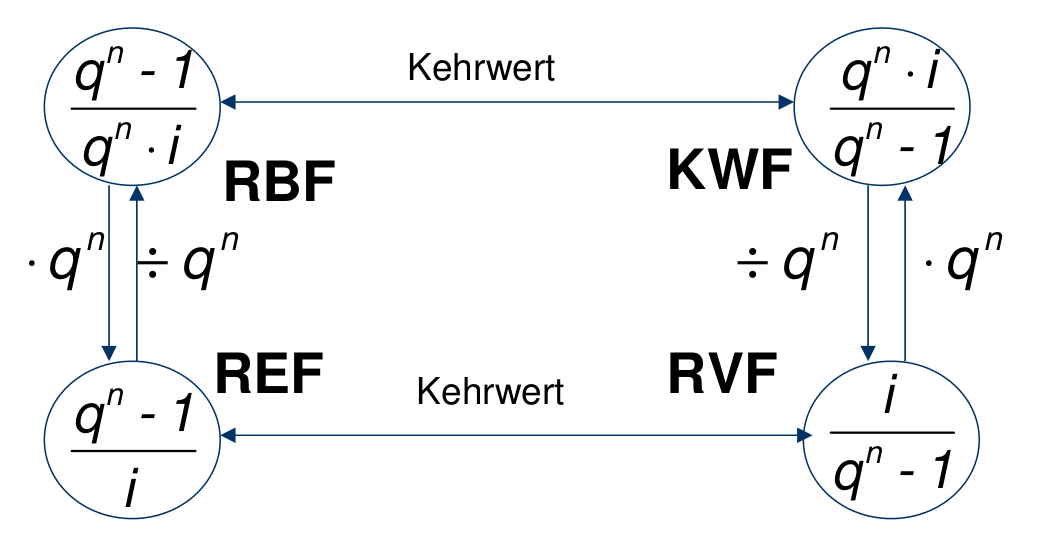
\includegraphics[height=4cm]{RentenUndKapitalfaktoren.png}

\begin{description}
	\item[Anlage 1] $- 200' + 120' \cdot \frac{1.10^3 - 1}{1.10^3 \cdot 0.1} \approx 98.4222'$
	\item[Anlage 2] $- 220' + 480' \cdot \frac{1}{1.10^4} \approx 107.8465'$
	\item[Anlage 3] 0, weil Standardoption (Interner Zinsfuß oder so)
\end{description}
Der Verein sollte sich also für Anlage 2 entscheiden (duh!).

\subsection{Investitionsrechnung}
Helmut B. plant die Eröffnung einer Druckerei. Dafür ist die Anschaffung einer Buchpresse erforderlich. Nachdem er Angebote eingeholt hat, stehen folgende Pressen, die jeweils 5 Jahre genutzt werden sollen, in der engeren Auswahl:

\vspace{\baselineskip}
\begin{tabular}{l|r|r}
	& Presse 1 & Presse 2 \\ \hline
	Anschaffungskosten (\euro) & 450.000 & 300.000 \\
	sonstige fixe Kosten (\euro) p.a. & 15.000 & 12.000 \\
	variable Kosten (\euro \ pro Verpackungseinheit) & 22 & 25 \\
	Restverkaufserlös (\euro) & 80.000 & 50.000
\end{tabular}

\vspace{\baselineskip}
Herr B. geht davon aus, 14.000 Verpackungseinheiten mit jeweils 20 Büchern verkaufen zu können und rechnet mit 5\% Zinsen.

\begin{enumerate}
	\item Welche Presse ist nach Kostenvergleichsrechnung die bessere Wahl? \\
		\begin{tabular}{lr|r}
			Abschreibung & $\frac{450.000 - 80.000}{5} = 74.000$ & $\frac{300.000 - 50.000}{5} = 50.000$ \\
			Kalkulatorischer Zins & $\frac{450.000 + 80.000}{2} \cdot 0.05 = 13.250$ & $\frac{300.000 + 50.000}{2} \cdot 0.05 = 8.750$ \\
			Sonstige Fixkosten & 15.000 & 12.000 \\
			Variable Kosten & $14.000 \cdot 22 = 308.000$ & $14.000 \cdot 25 = 350.000$ \\ \hline
			$\sum$ & 410.250 & 420.750
		\end{tabular}
		\vspace{\baselineskip} \\
		Er sollte sich also für Presse 1 entscheiden.
	\item Bei welcher Produktionsmenge an Verpackungseinheiten sind beide Pressen gleich gut?
		\begin{align*}
		\underbrace{410.250}_{\text{Kosten pro Jahr}} - \underbrace{308.000}_{\text{variable Kosten}} &= \underbrace{102.250}_{\text{Fixe Kosten}} \tag{Maschine 1} \\
		\underbrace{420.750}_{\text{Kosten pro Jahr}} - \underbrace{350.000}_{\text{variable Kosten}} &= \underbrace{70.750}_{\text{Fixe Kosten}} \tag{Maschine 2} \\
		\text{Fixkosten}_1 + \text{variable Kosten}_1 &\overset{!}{=} \text{Fixkosten}_2 + \text{variable Kosten}_2 \\
		102.250 + 22 \cdot x &= 70.750 + 25 \cdot x \\
		x &= 10.500
		\end{align*}
	\item Da Presse 1 zusätzlich noch das Gesicht des Charmanten Herrn B. auf das Cover drucken kann, rechnet her hier mit einem Verkaufspreis von 18\euro \ je Buch, bei Presse 2 jedoch nur mit 16\euro \ je Buch. Für welche Presse entscheidet er sich nach einer Gewinnvergleichsrechnung? Wir nehmen dabei an, dass Presse 1 Kosten von 410.000 \euro \ und Presse 2 Kosten von 420.000 \euro \ verursacht (Vermeidung von Folgefehlern).
	
		\vspace{\baselineskip}
		\begin{tabular}{l|r|r}
			& Presse 1 & Presse 2 \\ \hline
			Erlös & $18 \cdot 20 \cdot 14.000 =5.040.000$ & $16 \cdot 20 \cdot 14.000 = 4.480.000$ \\
			Kosten & 410.000 & 420.000 \\ \hline
			Gewinn & 4.630.000 & 4.060.000
		\end{tabular}
		
		\vspace{\baselineskip}
		Die Presse 1 bietet einen höheren Gewinn, daher wird man sich für diese entscheiden.
\end{enumerate}

\subsection{Äquivalenzziffernrechnung}
Der Lebensmittelhersteller Krafft vertreibt 4 Sorten Energy-Drinks. Die Kosten pro Palette ergeben sich zum Großteil aus der Herstellungsdauer. Die folgende Tabelle sind die Herstellungszahlen und Produktionszeiten pro Palette und Typ angegeben. Die gesammten Herstellungskosten betragen 320.000 \euro.

\begin{tabular}{lcc}
	Energy-Drink & Produktionszahlen (in Paletten) & Hertellungsdauer (in Minuten) \\ \hline
	Ungehäuer & 2400 & 24 \\
	Red Donkey & 1200 & 32 \\
	Rhinozeros & 600 & 18 \\
	Rockikone & 2000 & 20
\end{tabular}

\vspace{\baselineskip}
Wie groß sind die Herstellungskosten in vollen Tausend \euro \ pro Produkttyp, wenn man die einstufige Äquivalenzziffernrechnung anwendet?

\vspace{\baselineskip}
\begin{tabular}{lrrrrr}
	Energy-Drink & Paletten & Minuten & Palettenminuten & Äquivalenzziffer & Kosten \\ \hline
	Ungehäuer & 2400 & 24 & 57600 & 0.3924 & 125' \\
	Red Donkey & 1200 & 32 & 38400 & 0.2616 & 83' \\
	Rhinozeros & 600 & 18 & 10800 & 0.0736 & 23' \\
	Rockikone & 2000 & 20 & 40000 & 0.2725 & 87' \\ \hline
	$\sum$ & & & 146800 & 1.0001 & 318'
\end{tabular}

\newpage
\section{Sonstiges}
\subsection{Binäre Zahlen}
Welche Dezimalzahlen entsprechen den folgenden Binärzahlen?
\begin{enumerate}
	\item
		\begin{tabular}{l|l|l}
			110 & 1010 & 10001 \\ \hline
			$6_d$ & $10_d$ & $17_d$
		\end{tabular}
	\item
		\begin{tabular}{l|l|l}
			11101 & 100100 & 1110001101 \\ \hline
			$29_d$ & $26_d$ & $909_d$
		\end{tabular}
\end{enumerate}
Schreibe folgende Dezimalzahlen im Binärsystem
\begin{enumerate}
	\item
		\begin{tabular}{l|l|l|l|l}
			1 & 2 & 4 & 8 & 16 \\ \hline
			$1_b$ & $10_b$ & $100_b$ & $1000_b$ & $10000_b$
		\end{tabular}
	\item
		\begin{tabular}{l|l|l}
			3 & 7 & 15 \\ \hline
			$11_b$ & $111_b$ & $1111_b$
		\end{tabular}
	\item
		\begin{tabular}{l|l|l|l}
			5 & 11 & 28 & 42\\ \hline
			$101_b$ & $1011_b$ & $11100_b$ & $101010_b$
		\end{tabular}
\end{enumerate}
Führe folgende Berechnungen durch
\begin{enumerate}
	\item $1101_b + 110_b = 10011_b$
	\item $1011101_b + 1001_b = 1100110_b$
	\item $1011101_b - 1001_b = 1010100_b$
	\item $1101_b - 110_b = 111_b$
	\item $1101_b \cdot 110_b = 1001110_b$
	\item $1011101_b \cdot 1001_b = 1101000101_b$
\end{enumerate}

\subsection{Modulare Arithmetik}
Was ist das Ergebnis folgender Rechnungen?
\begin{enumerate}
	\item $3 \bmod 3 \equiv 0$
	\item $7 \bmod 3 \equiv 1$
	\item $13 \bmod 5 \equiv 3$
\end{enumerate}
Wozu sind die folgenden Terme äquivalent?
\begin{enumerate}
	\item $3 + 4 \pmod 2 \equiv 1$
	\item $12 + 1 \pmod 5 \equiv 3$
	\item $4 \cdot 5 \pmod 7 \equiv 6$
	\item $3 \cdot 8 \pmod {11} \equiv 2$
\end{enumerate}
Welches x löst die Gleichung?
\begin{enumerate}
	\item $0 + x \equiv 3 \pmod 5 \rightarrow x \equiv 3$
	\item $1 + x \equiv 0 \pmod 5 \rightarrow x \equiv 4$
	\item $4 + x \equiv 2 \pmod 5 \rightarrow x \equiv 3$
\end{enumerate}

\end{document}









